% Paquets généraux
\documentclass[a4paper,12pt,titlepage,twoside]{article}
\usepackage[T1]{fontenc}
\usepackage[utf8]{inputenc}
\usepackage[french]{babel}
\addto\captionsfrench{%
  \renewcommand{\tablename}{Tableau}%
}
\usepackage[gen]{eurosym}
%\usepackage[dvips]{graphicx}
\usepackage{fancyhdr}
\usepackage{pdfpages} 
\usepackage{multido}
\usepackage{hyperref}
%\usepackage{textcomp}
\usepackage{schemabloc}
\usepackage[bitstream-charter]{mathdesign}
\usepackage{array}
\newcolumntype{P}[1]{>{\centering\arraybackslash}p{#1}}

\newcommand{\id}{54}
\newcommand{\nom}{Liaisons mécaniques}
\newcommand{\sequence}{04}
\newcommand{\num}{01}
\newcommand{\type}{TP}
\newcommand{\descrip}{Modélisation d'un solide. Comportement des liaisons mécaniques. Modéliser les mécanismes du laboratoire par un schéma cinématique, paramétré.}
\newcommand{\competences}{A3-C4: Analyse d'architecture et de comportement \\ &  Mod1-C1: Isolement d'un solide ou d'un système de solides \\ &  Mod2-C10-1: Modèle de solide indéformable \\ &  Mod2-C11: Modélisation géométrique et cinématique des mouvements entre solides indéformables \\ &  Mod2-C12: Modélisation cinématique des liaisons entre solides \\ &  Mod2-C15: Modélisation des actions mécaniques \\ &  Rés-C6: Utilisation d'un solveur ou d'un logiciel multi physique \\ &  Com1-C1: Différents descripteurs introduits dans le programme \\ &  Com2-C4: Outils de communication}
\newcommand{\nbcomp}{9}
\newcommand{\systemes}{Plateforme Stewart}
\newcommand{\systemessansaccent}{Plateforme Stewart}
\newcommand{\ilot}{2}
\newcommand{\ilotstr}{02}
\newcommand{\dossierilot}{\detokenize{Ilot_02 Plateforme Stewart}}
\newcommand{\imageun}{Plateforme}

\newcommand{\urlsysteme}{\href{https://www.costadoat.fr/systeme/57}{Ressources système}}
\newcommand{\matlabsimscape}{\href{https://github.com/Costadoat/Sciences-Ingenieur/raw/master/Systemes/Plateforme Stewart/Plateforme_Stewart_Simscape.zip}{Modèle Simscape}}
\newcommand{\solidworks}{\href{https://github.com/Costadoat/Sciences-Ingenieur/raw/master/Systemes/Plateforme Stewart/Plateforme_Stewart_Solidworks.zip}{Modèle Solidworks}}
\newcommand{\edrawings}{\href{https://github.com/Costadoat/Sciences-Ingenieur/raw/master/Systemes/Plateforme Stewart/Plateforme_Stewart.EASM}{Modèle eDrawings}}
\newcommand{\test}{Stewart_param1}
\newcommand{\testi}{Stewart_param2}
\newcommand{\testii}{Stewart_param3}
\newcommand{\testiii}{Stewart_param4}
\newcommand{\testiiii}{Stewart_euler}

\newcommand{\institute}{Lycée Dorian}

\usepackage{fancyvrb}
\usepackage{color}
\usepackage{xcolor}
\usepackage{colortbl}
\usepackage{helvet}
\renewcommand{\familydefault}{\sfdefault}
\usepackage{amsfonts}
\usepackage{amsmath}
%\usepackage{xspace}
\usepackage{varioref}
\usepackage{tabularx}
%\usepackage{floatflt}
\usepackage{graphics}
\usepackage{wrapfig}
\usepackage{textcomp}
\usepackage{tikz}
\usepackage{wrapfig}
\usepackage{gensymb}
\usepackage[percent]{overpic}
\usepackage[european]{circuitikz}
\usetikzlibrary{babel}
\usepackage{ifthen}
\usepackage{cancel}
\usepackage{etoolbox}
\usepackage{multirow}
%\usepackage{boxedminipage}
\definecolor{gris25}{gray}{0.75}
\definecolor{bleu}{RGB}{18,33,98}
\definecolor{bleuf}{RGB}{42,94,171}
\definecolor{bleuc}{RGB}{231,239,247}
\definecolor{rougef}{RGB}{185,18,27}
\definecolor{rougec}{RGB}{255,188,204}%255,230,231
\definecolor{vertf}{RGB}{103,126,82}
\definecolor{vertc}{RGB}{220,255,191}
\definecolor{forestgreen}{rgb}{0.13,0.54,0.13}
\definecolor{blcr}{rgb}{0.59,0.69,0.84}
\definecolor{blfr}{rgb}{0.32,0.51,0.75}
\definecolor{orfr}{rgb}{0.90,0.42,0.15}
\definecolor{orcr}{rgb}{0.90,0.65,0.50}
\definecolor{orangef}{rgb}{0.659,0.269,0.072}
\definecolor{orange}{rgb}{0.58,0.35,0.063}
\definecolor{orangec}{rgb}{0.43,0.32,0.25}
\definecolor{rcorrect}{rgb}{0.6,0,0}
\definecolor{sequence}{rgb}{0.75,0.75,0.75}
\definecolor{competences}{rgb}{0.61,0.73,0.35}
\definecolor{grisf}{HTML}{222222}
\definecolor{grisc}{HTML}{636363}
\definecolor{normal}{HTML}{4087c4}
\definecolor{info}{HTML}{5bc0de}
\definecolor{success}{RGB}{92,184,92}
\definecolor{warning}{RGB}{240,173,78}
\definecolor{danger}{RGB}{217,83,79}
\hypersetup{                    % parametrage des hyperliens
    colorlinks=true,                % colorise les liens
    breaklinks=true,                % permet les retours à la ligne pour les liens trop longs
    urlcolor= blfr,                 % couleur des hyperliens
    linkcolor= orange,                % couleur des liens internes aux documents (index, figures, tableaux, equations,...)
    citecolor= forestgreen                % couleur des liens vers les references bibliographiques
    }

% Mise en page
\pagestyle{fancy}

\setlength{\hoffset}{-18pt}
\setlength{\oddsidemargin}{0pt} 	% Marge gauche sur pages impaire2s
\setlength{\evensidemargin}{0pt} 	% Marge gauche sur pages paires
\setlength{\marginparwidth}{00pt} 	% Largeur de note dans la marge
\setlength{\headwidth}{481pt} 	 	% Largeur de la zone de tête (17cm)
\setlength{\textwidth}{481pt} 	 	% Largeu\textbf{r de la zone de texte (17cm)
\setlength{\voffset}{-18pt} 		% Bon pour DOS
\setlength{\marginparsep}{7pt}	 	% Séparation de la marge
\setlength{\topmargin}{-30pt} 		% Pas de marge en haut
\setlength{\headheight}{55pt} 		% Haut de page
\setlength{\headsep}{20pt} 		% Entre le haut de page et le texte
\setlength{\footskip}{30pt} 		% Bas de\textbf{ page + séparation
\setlength{\textheight}{700pt} 		% Hauteur de l'icone zone de texte (25cm)
\setlength\fboxrule{1 pt}
\renewcommand{\baselinestretch}{1}
\setcounter{tocdepth}{1}
\newcommand{\cadre}[2]
{\fbox{
  \begin{minipage}{#1\linewidth}
   \begin{center}
    #2\\
   \end{center}
  \end{minipage}
 }
}

\newcommand{\repon}[1]
{
~\ \\
\begin{tabular}{|m{\linewidth}|}
 \hline
\multido{}{#1}{\\ \hline}
\end{tabular}
}

\newcounter{num_quest} \setcounter{num_quest}{0}
\newcounter{num_rep} \setcounter{num_rep}{0}
\newcounter{num_cor} \setcounter{num_cor}{0}

\newcommand{\question}[1]{\refstepcounter{num_quest}\par
~\ \\ \parbox[t][][t]{0.15\linewidth}{\textbf{Question \arabic{num_quest}}}\parbox[t][][t]{0.85\linewidth}{#1}\par
}


\newcommand{\reponse}[3]
{\refstepcounter{num_rep}
\noindent
\rule{\linewidth}{.5pt}\\
\textbf{Question \arabic{num_rep}:} ~\ \\
\ifdef{\public}{\multido{\i=1+1}{#1}{~\ \\}#2}{#3}
}

\newcommand{\cor}
{\refstepcounter{num_cor}
\noindent
\rule{\linewidth}{.5pt}
\textbf{Question \arabic{num_cor}:} \\
}

\newcommand{\repcarre}[2]
{
~\ \\
\begin{tikzpicture}
\draw [fill=white] (0,0) rectangle +(\linewidth,#1);
\node[align=left] at (1.1,#2-0.3) {\textbf{Question #1:}};
\end{tikzpicture}
}

\newcommand{\titre}[1]
{\begin{center}
\cadre{0.8}{\huge #1} 
\end{center}
}


% En tête et pied de page
\lhead{\nom}
\rhead{
\includegraphics[width=2cm]{../../img/logo}}
\lfoot{\auteurun,\ \auteurdeux}
\cfoot{Page \thepage}

\fancypagestyle{documentreponse}{%
  \fancyhf{}
  \fancyhead[LO]{Nom: ........................ Prénom: ........................}
  \fancyhead[LE]{\nom}
  \fancyhead[RE,RO]{
\includegraphics[width=2cm]{../../img/logo}}
  \lfoot{Document réponse}
  \cfoot{Page \thepage}
   }
  
\fancypagestyle{correction}{%
  \fancyhf{}
  \lhead{\colorbox{danger}{\begin{minipage}{0.65\paperwidth} \textcolor{white}{\textbf{Correction}} \end{minipage}} }
  \rhead{
\includegraphics[width=2cm]{../../img/logo}}
  \lfoot{Renaud Costadoat, Françoise Puig}
  \rfoot{\colorbox{danger}{\begin{minipage}{0.5\paperwidth} \begin{flushright}\textcolor{white}{\textbf{Correction}}\end{flushright} \end{minipage}} }}

\fancypagestyle{correctioninfo}{%
  \fancyhf{}
  \lhead{\colorbox{danger}{\begin{minipage}{0.65\paperwidth} \textcolor{white}{\textbf{Correction}} \end{minipage}} }
  \rhead{
\includegraphics[width=2cm]{../../img/logo}}
  \lfoot{Renaud Costadoat, Juliette Genzmer, Willie Robert}
  \rfoot{\colorbox{danger}{\begin{minipage}{0.6\paperwidth} \begin{flushright}\textcolor{white}{\textbf{Correction}}\end{flushright} \end{minipage}} }}

\renewcommand{\footrulewidth}{0.4pt}

\usepackage{eso-pic}
\newcommand{\BackgroundPic}{%
\put(0,0){%
\parbox[b][\paperheight]{\paperwidth}{%
\vfill
\begin{center}
\hspace{0.5cm}\vspace{0.5cm}

\includegraphics[width=\paperwidth,height=\paperheight,%
keepaspectratio]{../../img/fond3}%
\end{center}
\vfill
}}}

\newcommand{\BackgroundPicdeux}{%
\put(25,-30){%
\parbox[b][\paperheight]{\paperwidth}{%
\vfill
\begin{center}

\includegraphics[width=\paperwidth,height=\paperheight,%
keepaspectratio]{../../img/fond4}%
\end{center}
\vfill
}}}

\begin{document}

\pagestyle{empty}

\AddToShipoutPicture*{\BackgroundPic}


\includegraphics[width=2cm]{../../img/logo}

\Huge{DS \num\ - \sujet}

\vspace{1cm}

\ifdef{\prive}{\begin{center}\colorbox{danger}{\Huge{Avec Correction}}\end{center}}{}

\begin{center}
\centering\huge{PTSI}
\end{center}

\vspace{2cm}


\begin{center}
\centering\Large{\jour}
\end{center}

\vspace{2cm}

\normalsize

\tableofcontents

\newpage

\AddToShipoutPicture{\BackgroundPicdeux}

\pagestyle{fancy}

\begin{center}
\Huge \sujet
\end{center}


\normalsize

\section{Présentation (20 min)}

\subsection{Mise en situation}

\begin{figure}[ht!]
\begin{center}
 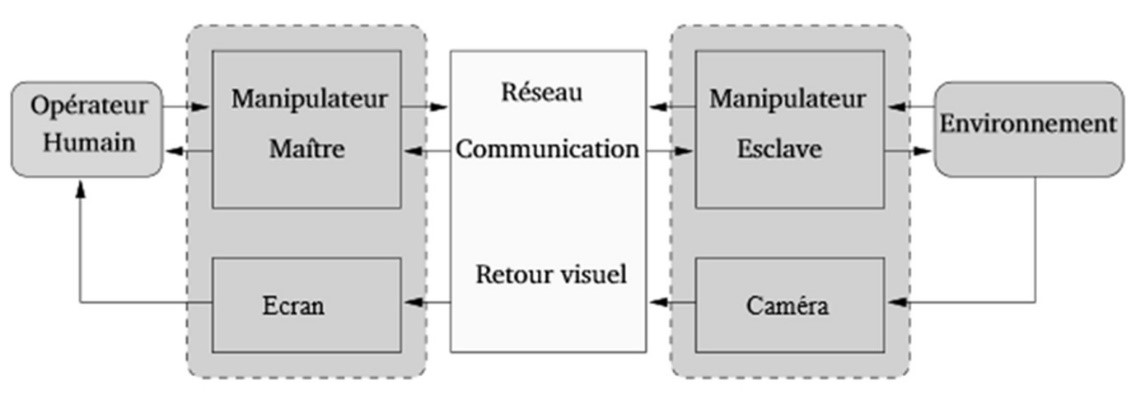
\includegraphics[width=0.9\linewidth]{img/Figure1}
\end{center}
\caption{Schéma de principe de la téléopération}
\label{fig1}
\end{figure}

Le cas d'utilisation étudié dans ce sujet est la téléopération sur organe mobile. Lors d'une opération, les organes sont soumis à des mouvements induits notamment par la respiration et les battements cardiaques. Lorsque le champ visuel est réduit, ces mouvements apportent une gêne au praticien qui doit les compenser manuellement.

\subsection{Nécessité d'un retour haptique}

Les dispositifs présentés et utilisés jusqu'à ce jour dans les hôpitaux sont des systèmes de téléopération unilatéraux : c'est-à-dire que l'information (généralement une position) ne circule que du maître vers l'esclave.

Dans ce cas, le manipulateur maître est généralement passif car il ne dispose d'aucune information sur l'environnement manipulé. De ce fait, il est très difficile d'évaluer l'effort appliqué aux organes. Le chirurgien ne peut s'appuyer que sur le retour visuel, sa connaissance anatomique et son expérience pour  opérer.

Différentes études ont démontré qu'il était beaucoup plus facile de réaliser certaines tâches quand l'utilisateur dispose d'informations haptiques. Le terme haptique est utilisé pour désigner le retour d'effort au sens kinesthésique mais également au sens tactile. Certains gestes de chirurgie, comme la dissection des tissus (25\% à 35\% du temps d'opération), ont été particulièrement analysés. Les résultats ont montré que le retour de force permet de limiter l'intensité et la durée des pics d'effort sur l'organe opéré.

Contrairement aux systèmes de téléopération unilatéraux qui peuvent être vus comme une succession de systèmes en boucle ouverte, les différents éléments des systèmes bilatéraux sont reliés par des boucles de contre-réaction et nécessitent une attention particulière (stabilité, précision, temps de réponse...).

\begin{figure}[ht!]
\begin{center}
 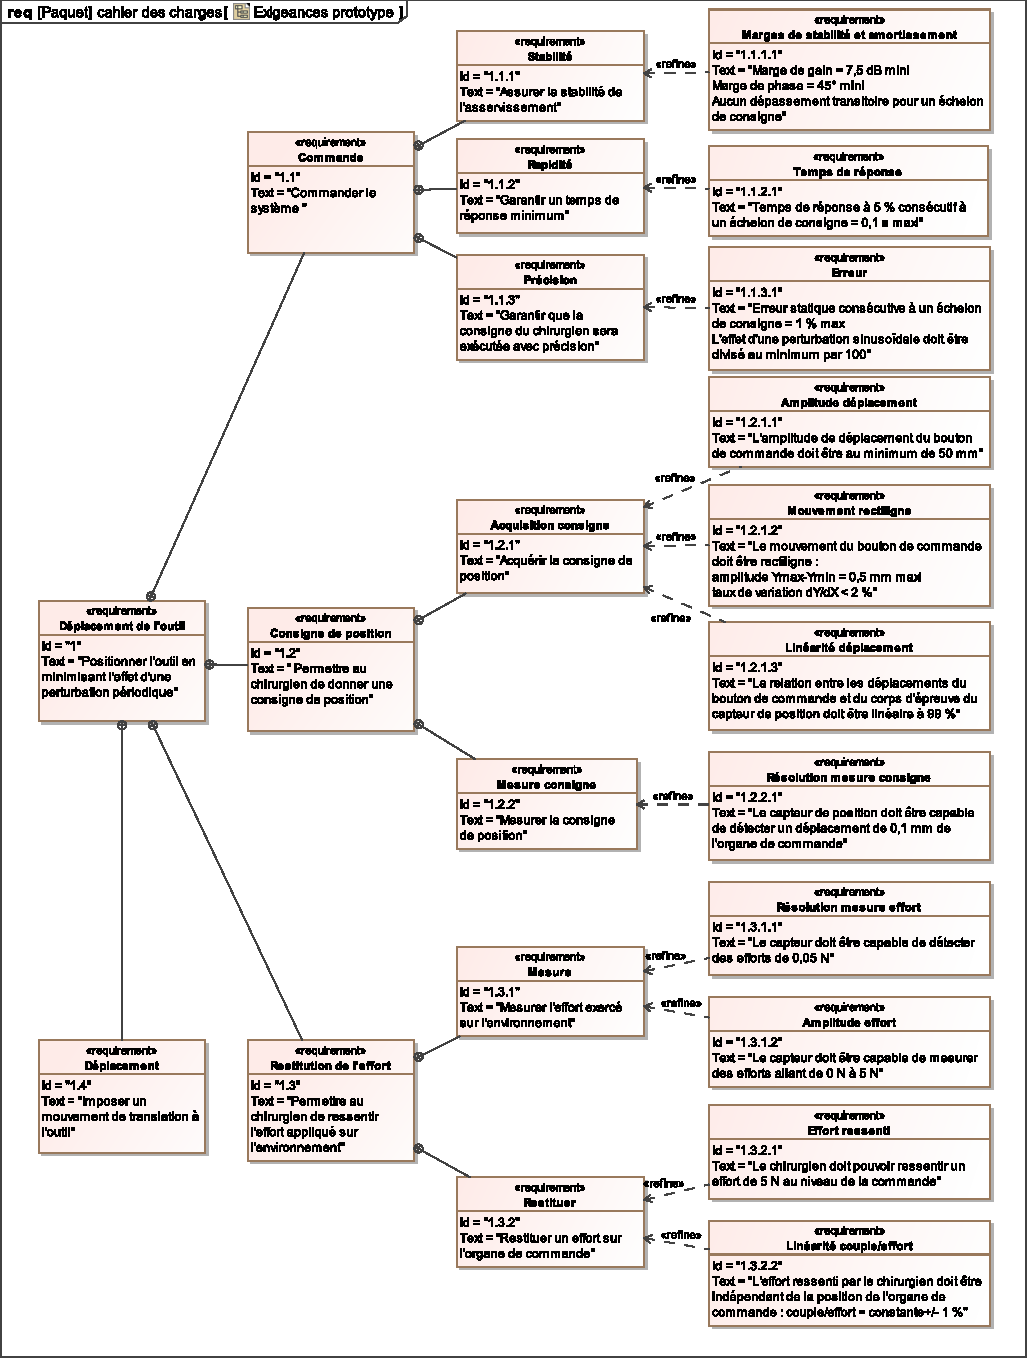
\includegraphics[width=0.98\linewidth]{img/Figure2}
\end{center}
\caption{Diagramme des exigences}
\label{fig2}
\end{figure}

\subsection{Problème posé}

Les effets du mouvement cardiaque sont négligeables lorsque la zone d'intérêt ne se situe pas dans le voisinage du c\oe ur. En revanche, les effets du mouvement respiratoire se propagent sur une grande partie des organes tels que les poumons, le diaphragme, le foie, les reins et le pancréas. Ils occasionnent une gêne importante en chirurgie abdominale.

Le dispositif expérimental étudié dans le sujet est réalisé à partir de 2 interfaces haptiques à 1 degré de liberté.

Objectif: L'objectif de cette étude est de concevoir et valider une commande permettant de rejeter une perturbation périodique.

\subsubsection{Démarche de résolution}

\begin{enumerate}
 \item Modélisation cinématique du manipulateur maître afin d'évaluer l'écart entre le déplace- ment simulé et le déplacement souhaité du levier de commande,
 \item Modélisation statique du manipulateur maître afin d'évaluer l'écart entre l'effort simulé et l'effort souhaité sur le levier de commande,
 \item Modélisation de l'environnement et mesure de l'écart généré par la conversion analogique numérique,
 \item Modélisation de la commande permettant d'annuler l'effet d'une perturbation sinusoïdale,
 \item Évaluation des écarts de performance entre le système modélisé, le système réel et  le
système souhaité.
\end{enumerate}

\section{Modélisation  du  manipulateur maître (50 min)}

\subsection{Diagramme de blocs internes}

\begin{figure}[ht!]
\begin{center}
 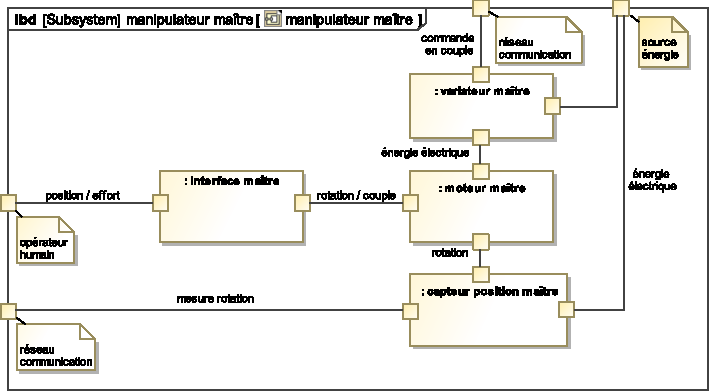
\includegraphics[width=0.9\linewidth]{img/Figure3}
\end{center}
\caption{Diagramme de blocs internes du manipulateur maître}
\label{fig3}
\end{figure}

Le manipulateur maître est constitué de :
\begin{itemize}
 \item une interface (mécanisme de HOEKEN) permettant de transformer le mouvement de
translation imposé par l'opérateur en mouvement de rotation,
 \item un variateur analogique asservi en courant permettant au moteur de restituer  un
couple précis,
 \item un moteur rotatif pour générer un retour d'effort sur l'opérateur humain,
 \item un capteur de position (codeur incrémental) pour mesurer la consigne de  position.
\end{itemize}

\subsection{Modélisation de l'interface maître}

Ce mécanisme est constitué de 4 barres reliées par des liaisons pivots.

\begin{figure}[ht!]
\begin{center}
\begin{minipage}{0.45\linewidth}
 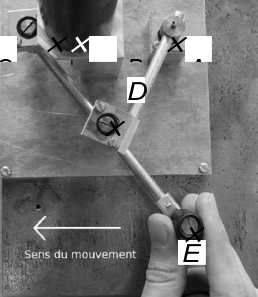
\includegraphics[width=0.8\linewidth]{img/Figure4}
 \caption{Mécanisme de HOEKEN}
 \label{fig4}
\end{minipage}\hfill
\begin{minipage}{0.45\linewidth}
 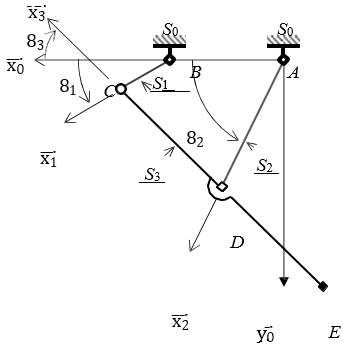
\includegraphics[width=0.8\linewidth]{img/Figure5}
 \caption{Modélisation cinématique}
 \label{fig5}
\end{minipage}
\end{center}
\end{figure}


\begin{table}[ht!]
\begin{center}
\begin{tabular}{|c|c|c|}
\hline
Solide & Repère associé	& Paramètres géométriques \\
\hline
$S_0$ (bâti AB)	& $R_0(A,\overrightarrow{x_0},\overrightarrow{y_0},\overrightarrow{z_0})$ & $\overrightarrow{AB}=L_0.\overrightarrow{x_0}$ avec $L_0 = 50mm$ \\
\hline
$S_1$ (barre BC) & $R_0(B,\overrightarrow{x_1},\overrightarrow{y_1},\overrightarrow{z_0})$ & $\overrightarrow{BC}=L_1.\overrightarrow{x_1}$  avec $L_1 = 25mm$ \\
 & & $\theta_1=(\overrightarrow{x_0},\overrightarrow{x_1})=(\overrightarrow{y_0},\overrightarrow{y_1})$ \\
$S_2$  (barre AD) & $R_0(B,\overrightarrow{x_2},\overrightarrow{y_2},\overrightarrow{z_0})$	& $\overrightarrow{AD}=L_2.\overrightarrow{x_2}$ avec $L_2 = 62,5 mm$ \\
 & & $\theta_2=(\overrightarrow{x_0},\overrightarrow{x_2})=(\overrightarrow{y_0},\overrightarrow{y_2})$ \\
\hline
$S_3$ (barre CDE) & $R_0(B,\overrightarrow{x_3},\overrightarrow{y_3},\overrightarrow{z_0})$ & $\overrightarrow{ED}=\overrightarrow{DC}=L_2.\overrightarrow{x_3}$ \\
 & & $\theta_3=(\overrightarrow{x_0},\overrightarrow{x_3})=(\overrightarrow{y_0},\overrightarrow{y_3})$ \\
\hline
\end{tabular}
 \caption{Paramétrage de l'interface maître}
 \label{tab1}
\end{center}
\end{table}


\subsubsection{Mesure de l'écart entre les performances géométriques souhaitées et simulées}

\paragraph{Objectif:} Vérifier que les exigences \og Amplitude déplacement \fg (Id 1.2.1.1), \og Mouvement rectiligne \fg (Id 1.2.1.2), \og Linéarité déplacement \fg (Id 1.2.1.3) peuvent être satisfaites par le mécanisme de HOEKEN.

\question{En développant une fermeture géométrique en projection dans la base du repère $R_0$, donner une relation algébrique reliant les paramètres $L_0$, $L_1$, $L_2$, $\theta_1$  et $\theta_3$.}

\question{De même, exprimer le vecteur position du point E ($\overrightarrow{AE}$) dans la base du repère $R_0$ en fonction de $L_0$, $L_1$, $L_2$, $\theta_1$  et $\theta_3$.}

La résolution analytique du système d'équations permettant d'obtenir le déplacement du point E en fonction de l'angle de rotation $\theta_1$ du moteur et des différentes longueurs du mécanisme n'étant pas triviale, seuls les résultats d'une simulation numérique seront analysés.

\begin{figure}[ht!]
\begin{center}
 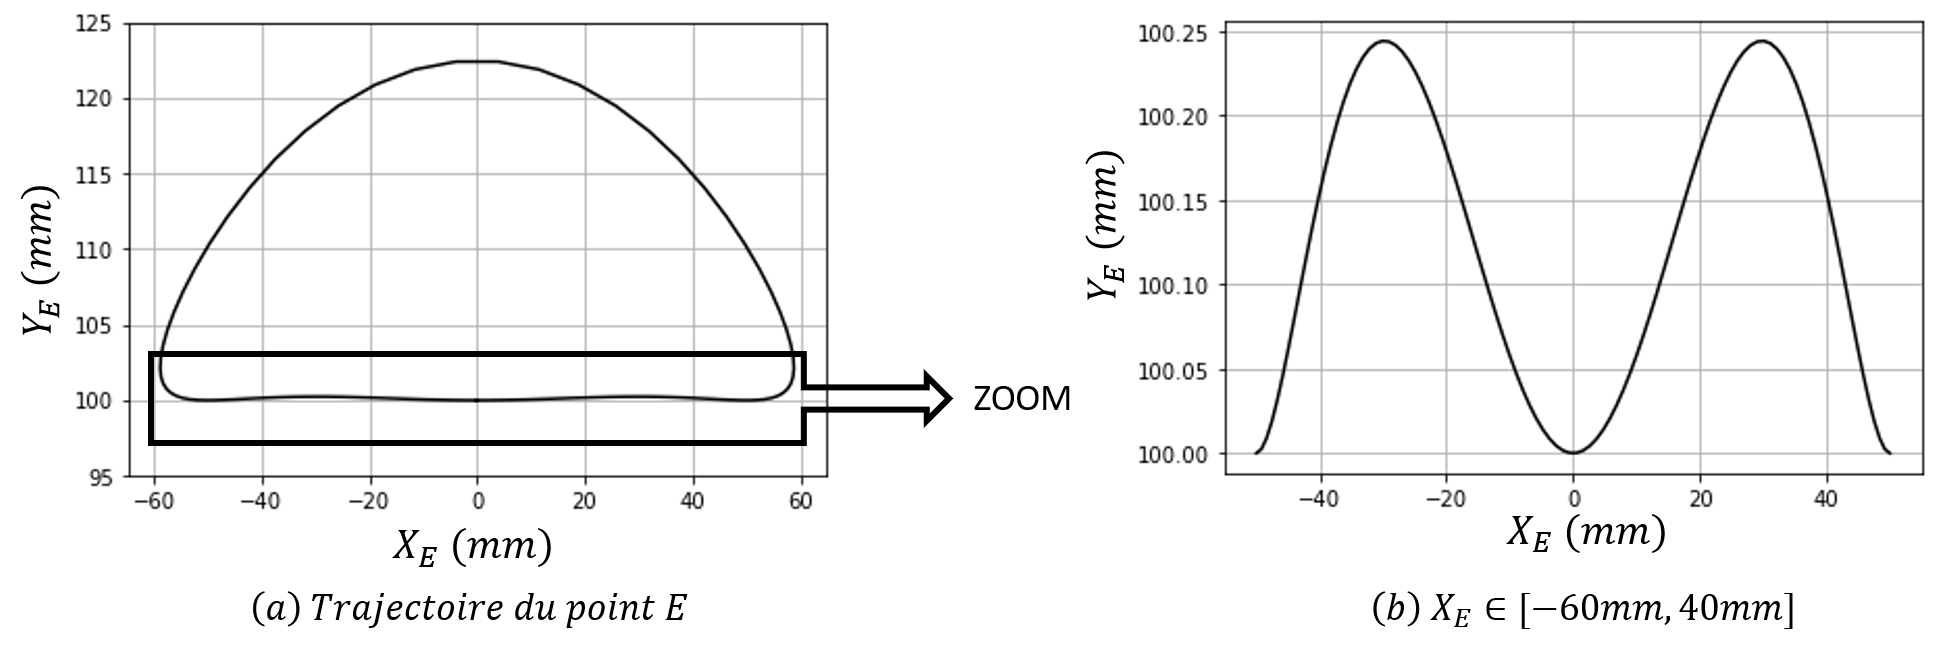
\includegraphics[width=0.9\linewidth]{img/Figure6}
  \caption{Trajectoire du point E dans le repère $R_0$}
 \label{fig6} 
 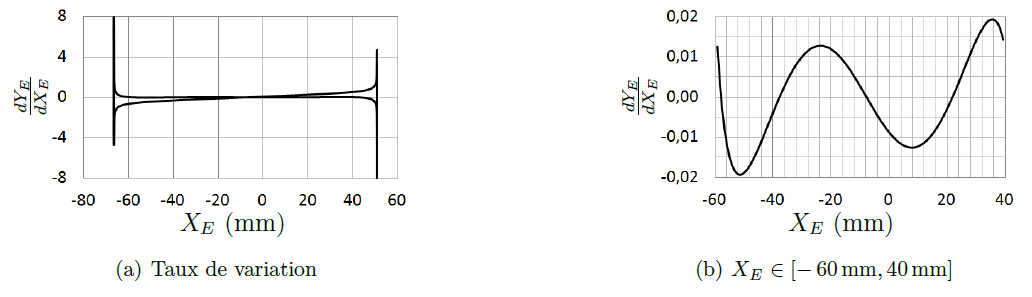
\includegraphics[width=0.9\linewidth]{img/Figure7}
  \caption{Taux de variation $\dfrac{dY_E}{dX_E}$ en fonction de l'abscisse du point E}
 \label{fig7} 
 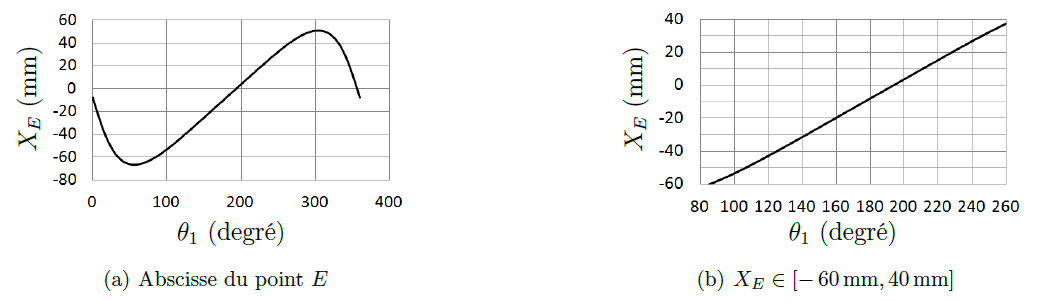
\includegraphics[width=0.9\linewidth]{img/Figure8}
  \caption{Abscisse du point E en fonction de la rotation de $\theta_1$}
 \label{fig8} 
 \end{center}
\end{figure}

\question{Vérifier que le déplacement du point $E$ est compatible avec les exigences \og Amplitude déplacement \fg (Id 1.2.1.1) et \og Mouvement rectiligne \fg (Id 1.2.1.2) sur l'intervalle $X_E\in[-60mm,40mm]$.}

\question{Proposer une démarche permettant de vérifier l'exigence \og Linéarité déplacement \fg (Id 1.2.1.3) sur l'intervalle $X_E\in[-60mm,40mm]$.}

\subsubsection{Mesure de l'écart entre les performances statiques souhaitées et simulées}

\paragraph{Objectif: }Vérifier que l'exigence \og Linéarité couple/effort \fg (id 1.3.2.2) peut être satisfaite par le mécanisme de HOEKEN.

\begin{itemize}
 \item On notera $\left\{T_{S_i\rightarrow S_j}\right\}=\left\{\begin{array}{cc}
 X_{ij} & L_{P,ij} \\
 Y_{ij} & M_{P,ij} \\
 Z_{ij} & N_{P,ij}
 \end{array}\right\}_{(P,B_0)}$ l'expression au point P, en projection dans la base $B_0$, du torseur de l'action mécanique exercée par le solide $S_i$ sur le solide $S_j$ ; toutes
les inconnues seront exprimées dans la base $B_0$.
 \item L'action mécanique exercée par le moteur sur $S_1$ sera modélisée par un couple $C_m(t).\overrightarrow{z_0}$.
 \item L'action mécanique exercée par l'opérateur sur $S_3$ sera modélisée par une force $F(t).\overrightarrow{x_0}$ appliquée au point E.
 \item L'accélération de la pesanteur sera représentée par le vecteur $\overrightarrow{g} = -g.\overrightarrow{z_0}$.
 \item Les inerties des solides en mouvement et les frottements dans les guidages seront négligés.
\end{itemize}

\question{Déterminer les équations algébriques issues du développement des 4 relations suivantes : \label{q5}}
\begin{itemize}
 \item Théorème du moment statique en B appliqué à l'équilibre de $S_1$, en projection sur $\overrightarrow{z_0}$.
 \item Théorème du moment statique en A appliqué à l'équilibre de $S_2$, en projection sur $\overrightarrow{z_0}$.
 \item Théorème du moment statique en D appliqué à l'équilibre de $S_3$, en projection sur $\overrightarrow{z_0}$.
 \item Théorème de la résultante statique appliqué à l'équilibre de $S_3$, en projection sur $\overrightarrow{y_2}$.
\end{itemize}

~\

Les équations élaborées à la question \ref{q5} permettent d'exprimer le couple moteur $C_m(t)$ en
fonction de l'action $F(t)$ exercée par l'opérateur :

\begin{center}
$C_m=\frac{L_1.F}{sin(\theta_2-\theta_3)}.(sin(\theta_1).sin(\theta_2+\theta_3)-2.cos(\theta_1).sin(\theta_2).sin(\theta_3))$
\end{center}

Cette relation n'étant pas linéaire, on propose à nouveau d'analyser les résultats d'une simulation numérique.

\begin{figure}[ht!]
\begin{center}
 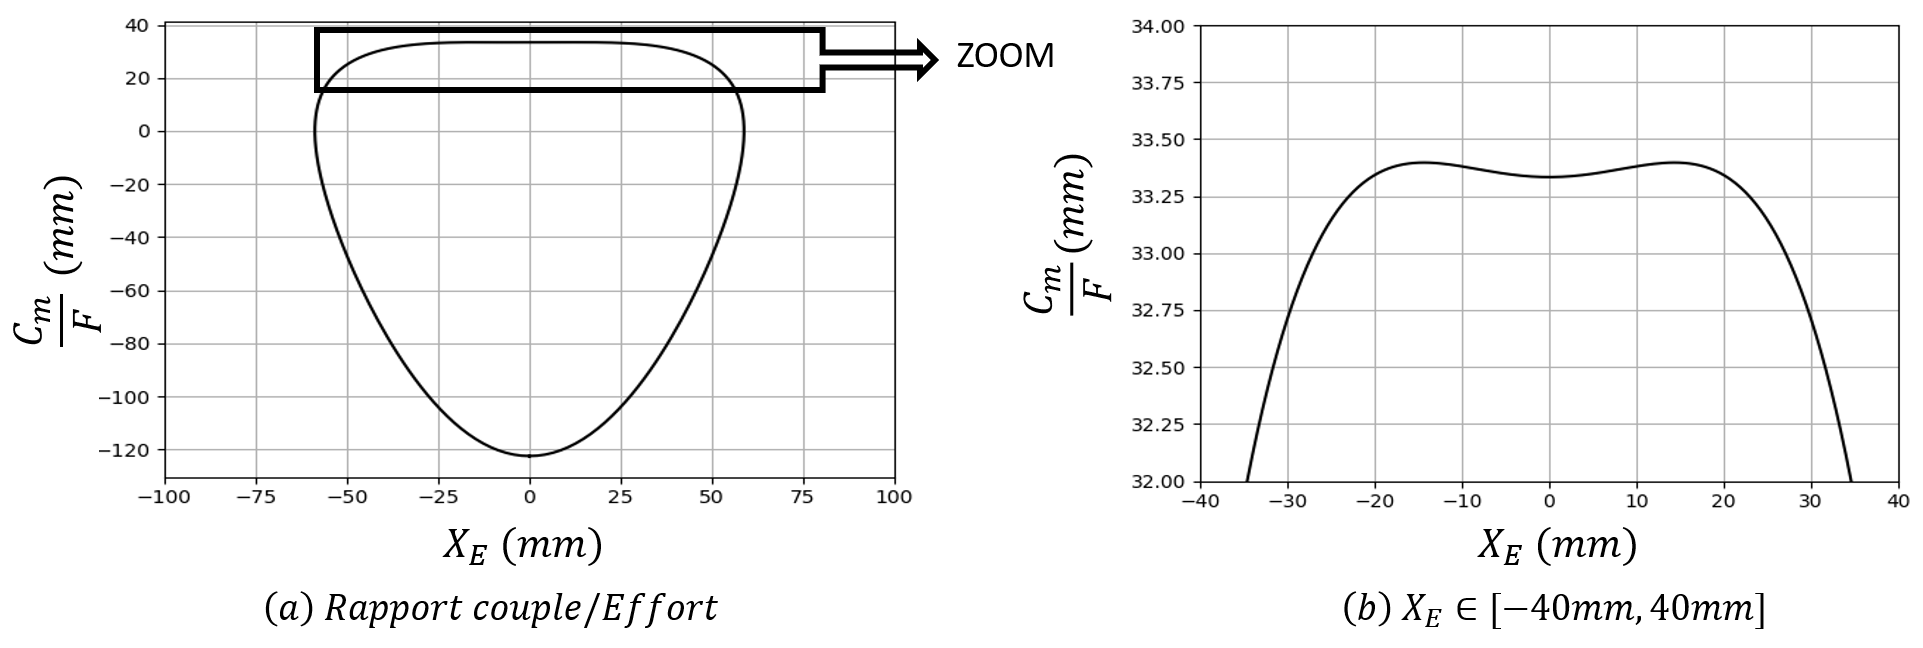
\includegraphics[width=0.9\linewidth]{img/Figure9b}
\end{center}
\caption{Couple moteur/effort opérateur en fonction de l'abscisse du point E}
\label{fig9b}
\end{figure}

\question{Déterminer, à partir de la figure \ref{fig9b}, sur quel intervalle de l'abscisse $X_E$ l'exigence \og Linéarité couple/effort \fg (id 1.3.2.2) est satisfaite. Indiquer si cet intervalle est compatible avec les exigences précédemment vérifiées.}

\subsection{Modélisation du codeur optique}

\paragraph{Objectif :} Vérifier que l'exigence « Résolution mesure consigne » (id 1.2.2.1) peut être satisfaite par ce codeur.

Un codeur incrémental est constitué d'un disque comportant 1 ou 2 voies avec éventuellement un index permettant de compter le nombre de tours (voir figure 10). Le disque est lié à
l'arbre tournant dont on souhaite connaître la position. D'un côté du disque se trouvent des
diodes électroluminescentes et de l'autre, des phototransistors.

Chaque voie du disque, excepté l'index, possède des zones alternativement opaques et transparentes. Le signal émis par le phototransistor, après un traitement électronique, est un signal
carré de type TTL (train d'impulsions plus ou moins espacées dans le temps).

\begin{figure}[ht!]
\begin{center}
 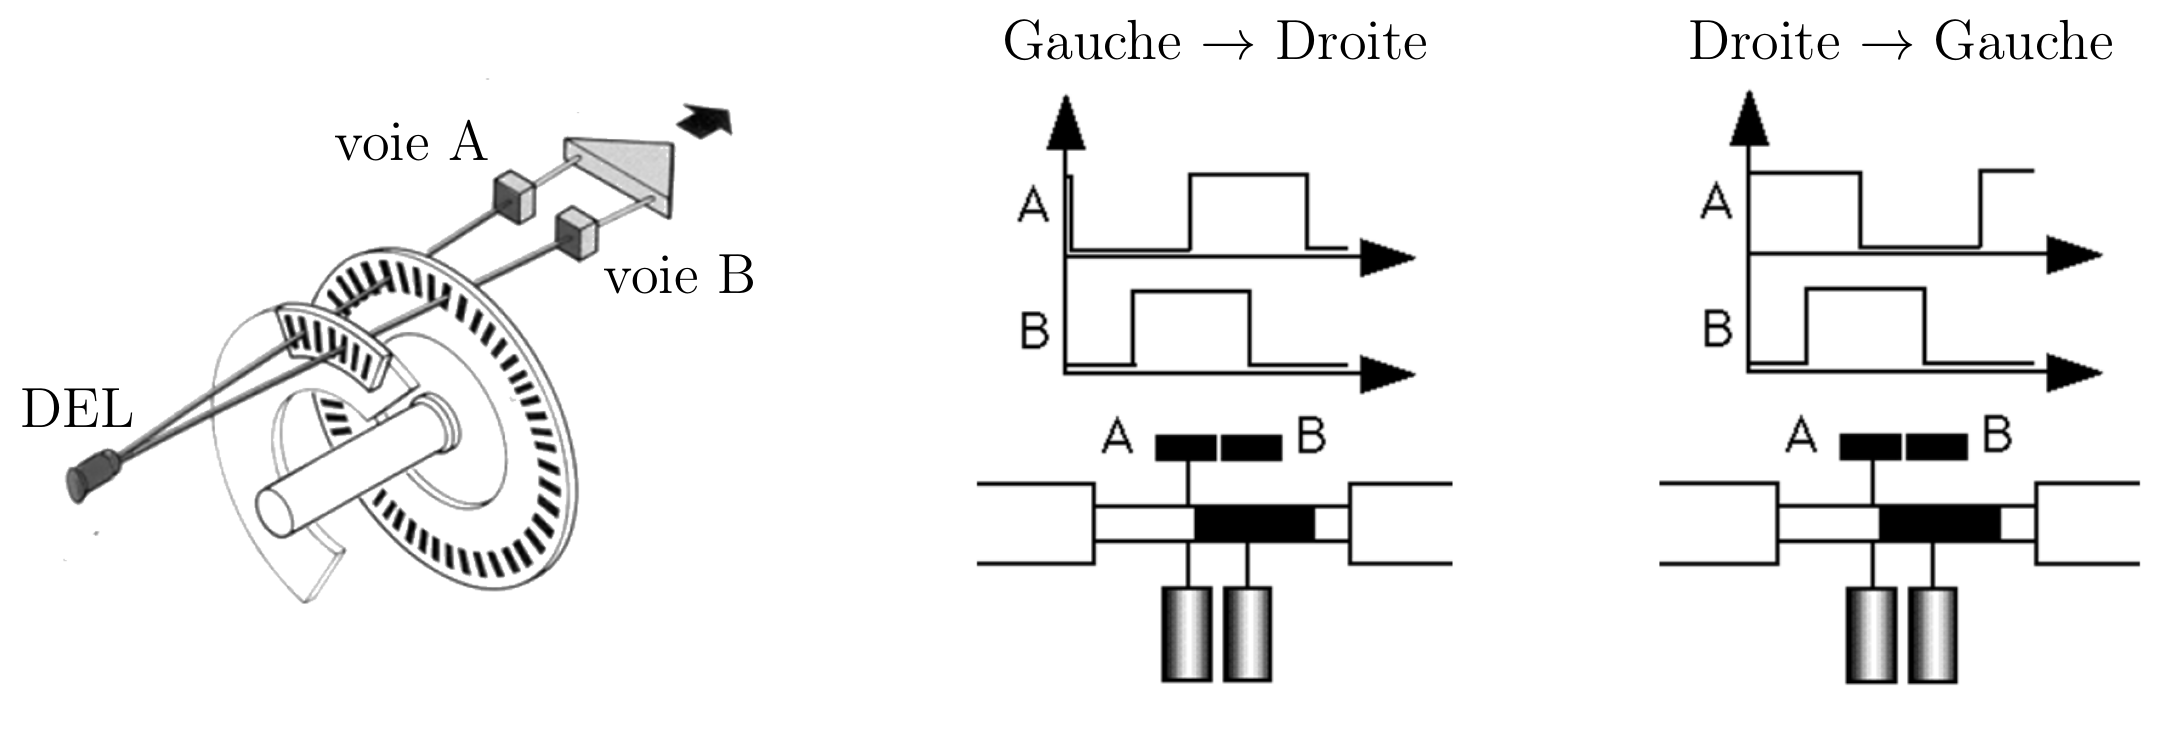
\includegraphics[width=0.9\linewidth]{img/Figure10b}
\end{center}
\caption{Principe de fonctionnement d'un codeur incrémental}
\label{fig10b}
\end{figure}

Le codeur utilisé pour mesurer l'angle moteur $\theta_1$ possède 1 piste de 1000 fentes et 2 détecteurs décalés d'1/2 fente. On notera A et B les variables logiques associées à ces 2 détecteurs.

\question{Sachant qu'une mesure est réalisée sur chaque front montant (passage de 0 à 1 d'une
variable) et front descendant (passage de 1 à 0 d'une variable), déterminer la résolution du
codeur. Vérifier la satisfaction de l'exigence \og Résolution mesure consigne \fg (id : 1.2.2.1).}

\section{Modélisation du manipulateur esclave (60 min)}

\subsection{Diagramme de blocs internes}

Le mécanisme de HOEKEN choisi pour l'interface maître réalise une bonne approximation de la trajectoire rectiligne mais ne permet pas une orientation constante du solide en mouvement. Cette solution n'est donc pas la plus appropriée pour mesurer (à l'aide d'un capteur) l'effort exercé par l'organe terminal.

\begin{figure}[ht!]
\begin{center}
 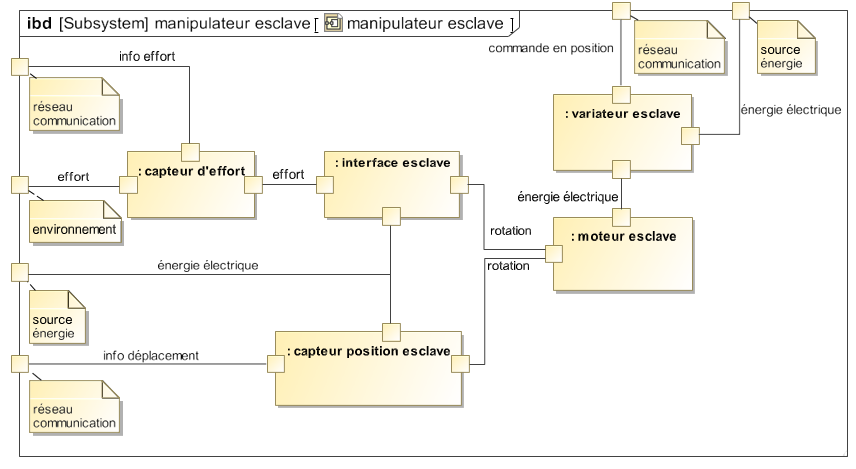
\includegraphics[width=0.9\linewidth]{img/Figure9}
\end{center}
\caption{Diagramme de blocs internes du manipulateur esclave}
\label{fig9}
\end{figure}

Le manipulateur esclave est constitué de :
\begin{itemize}
 \item une interface permettant de transformer le mouvement de rotation imposé par le moteur
en mouvement de translation rectiligne,
 \item un moteur rotatif pour générer le mouvement,
 \item un variateur analogique permettant de commander le moteur,
 \item un capteur de position (codeur incrémental) pour mesurer le déplacement de l'organe terminal,
 \item un capteur d'effort pour mesurer l'effort exercé par l'organe terminal sur  l'environnement.
\end{itemize}

\subsection{Modélisation de l'interface esclave (50 min)}

\begin{figure}[ht!]
\begin{center}
 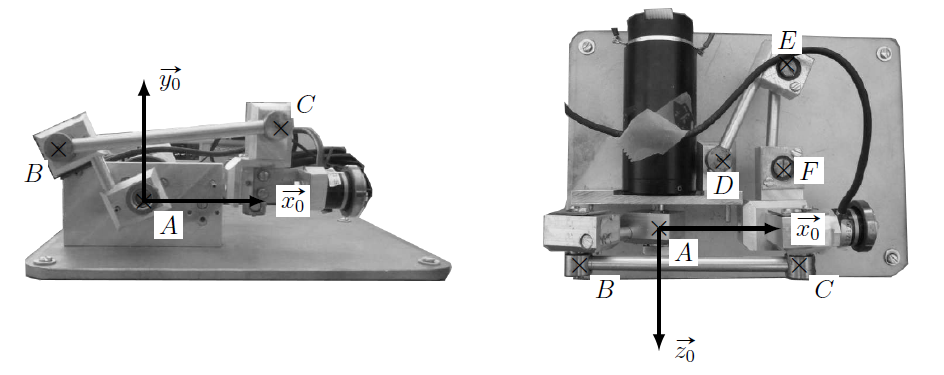
\includegraphics[width=0.9\linewidth]{img/Figure10}
\end{center}
\caption{L'interface esclave}
\label{fig10}
\end{figure}

\begin{figure}[ht!]
\begin{center}
 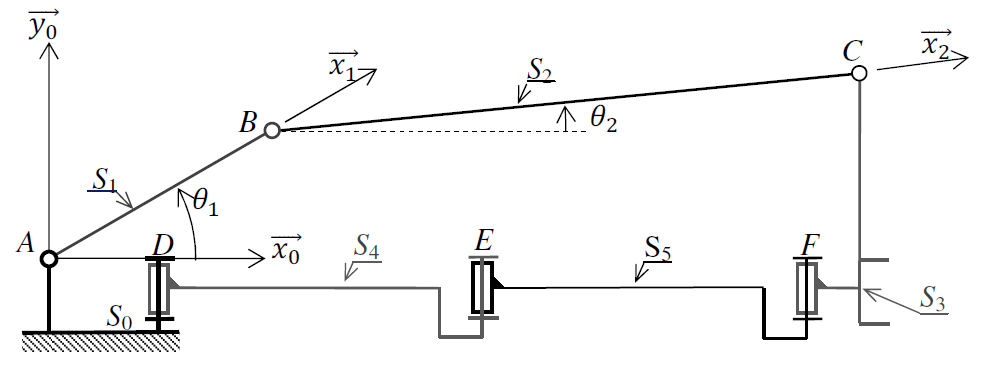
\includegraphics[width=0.9\linewidth]{img/Figure11}
\end{center}
\caption{Modélisation cinématique}
\label{fig11}
\end{figure}

Données:
\begin{itemize}
 \item Inertie	équivalente	ramenée	à l'axe $(A,\overrightarrow{z_0})$: $I_1=5,7\times 10^{-5}kg.m^2$,
 \item Frottement fluide entre rotor et stator : $f_v = 1,6\times 10^{-3} N.m.s$,
 \item Masse du solide 3 : $M_3=0,1kg$,
 \item Toutes les autres masses sont négligées.
\end{itemize}

Objectif: Modéliser le comportement de l'interface esclave de façon à évaluer son comportement au sein d'une boucle d'asservissement.

\question{Tracer le graphe des liaisons du dispositif esclave. Donner le degré d'hyperstatisme de la modélisation de ce mécanisme.}

\question{Proposer une modification simple pour le rendre isostatique.}

\question{Montrer que le mouvement de $S_3/S_0$ ne peut être qu'une translation de direction $\overrightarrow{x_0}$.}

\question{Déterminer $\overrightarrow{V_{C\in3/0}}$ en fonction de $\dot{\theta_1}$, $\theta_1$  et $\theta_2$.}

~\

Les paramètres dynamiques sont liés par l'équation différentielle suivante: \\ $(M_3+I_1.\alpha^2).\ddot{x_s}+f_v.\alpha^2.\dot{x_s}=C_m.\alpha$, avec $\alpha=-30m^{-1}$.

\question{Donner, en justifiant les hypothèses et théorèmes utilisés, sous forme canonique, la fonction de transfert modélisant le comportement dynamique du manipulateur esclave : $H(p)=\dfrac{X_s(p)}{C_m(p)}$ sachant que $X_s(p)=L[x_s(t)]$ et $C_m(p)=L[C_m(t)]$. Faire l'application numérique.}

\section{Réalisation de la commande de l'esclave (60min)}

\paragraph{Objectif :} Concevoir la commande du dispositif esclave de façon à satisfaire l'ensemble des exigences incluses dans l'exigence \og Commande \fg (Id 1.1).

\begin{figure}[ht!]
\begin{center}
 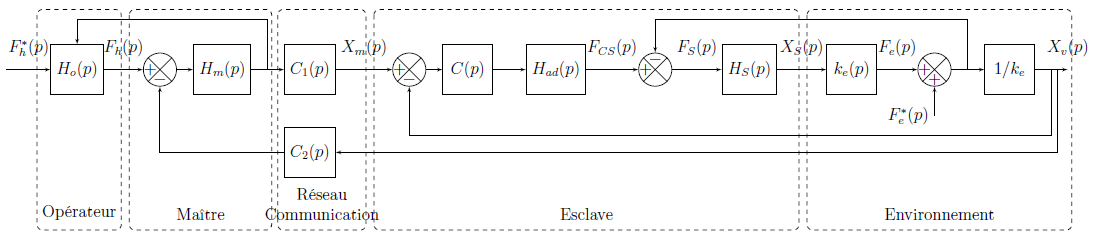
\includegraphics[width=0.9\linewidth]{img/Figure12}
\end{center}
\caption{Schéma bloc simplifié de la commande}
\label{fig12}
\end{figure}

\subsection{Modélisation de l'environnement}

\paragraph{Objectif :} Modéliser la perturbation liée à l'environnement.

Afin de modéliser la pénétration de l'aiguille dans les tissus, un essai a été réalisé sur l'organe d'un porc. La figure suivante montre le profil d'effort lors d'une insertion d'aiguille robotisée sur le foie d'un porc vivant anesthésié. Le déplacement du robot est représenté en pointillé et la force mesurée selon l'axe de l'aiguille en trait plein.
 
\begin{figure}[ht!]
\begin{center}
 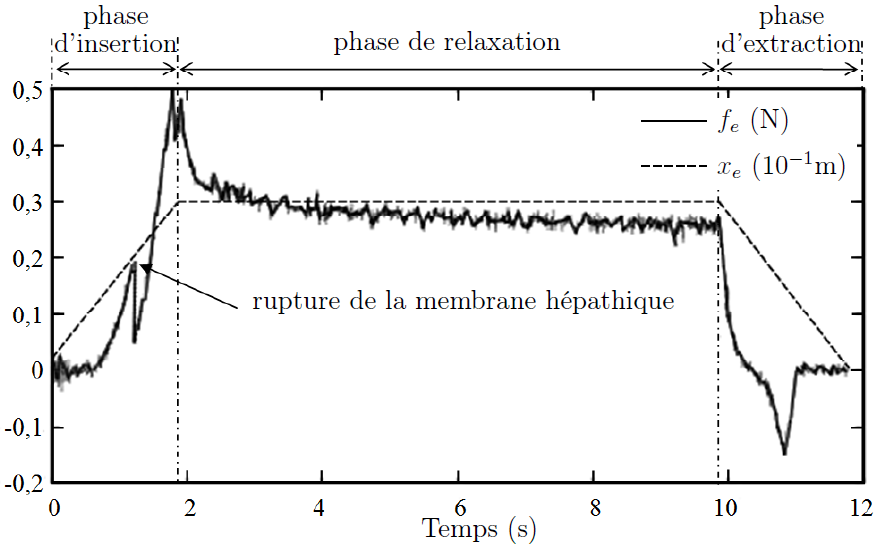
\includegraphics[width=0.7\linewidth]{img/Figure13}
\end{center}
\caption{Pénétration d'une aiguille dans le foie d'un porc}
\label{fig13}
\end{figure}

\question{\textbf{En considérant uniquement la fin de la phase d'insertion}, justifier le choix de modéliser (en première approche) l'effort de pénétration d'une aiguille dans un tissus par une fonction linéaire : $f_e(t) = k_e.x_e(t)$. Évaluer la valeur de $k_e$.}

Dans la suite du sujet, nous prendrons : $f_e(t)=k_e.x_e(t)$ avec $k_e=200N.m^{-1}$ qui correspond à une moyenne sur plusieurs organes.

Afin de modéliser les mouvements dûs à la respiration d'un patient, des mesures ont été effectuées. Elles représentent la position $x_e(t)$ de la partie supérieure de l'organe à opérer en fonction du temps.

\begin{figure}[ht!]
\begin{center}
 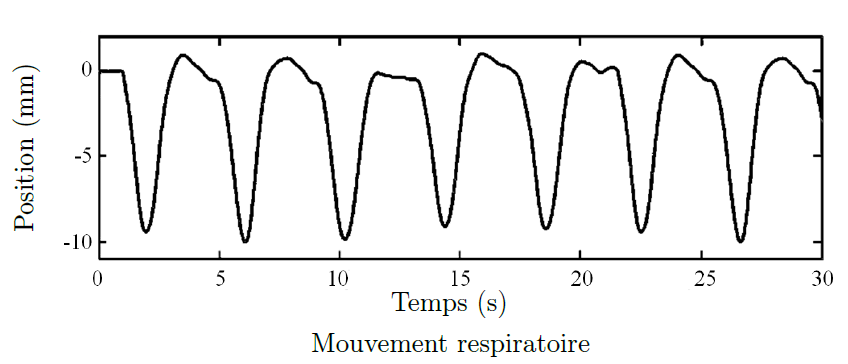
\includegraphics[width=0.7\linewidth]{img/Figure14}
\end{center}
\caption{Mouvement respiratoire}
\label{fig14}
\end{figure}

\question{Justifier la modélisation du déplacement par la fonction : $x_e(t)=A\left[-1+sin\left(2.\pi.f.t+\phi\right)\right]$ et donner les valeurs de $A$ et $f$. En déduire l'expression de $f_e(t)$.}

Pour simuler ce mouvement respiratoire, un dispositif composé d'un moteur linéaire, d'un ressort et d'un capteur d'effort est ajouté en sortie du manipulateur esclave (figure suivante).

\begin{figure}[ht!]
\begin{center}
 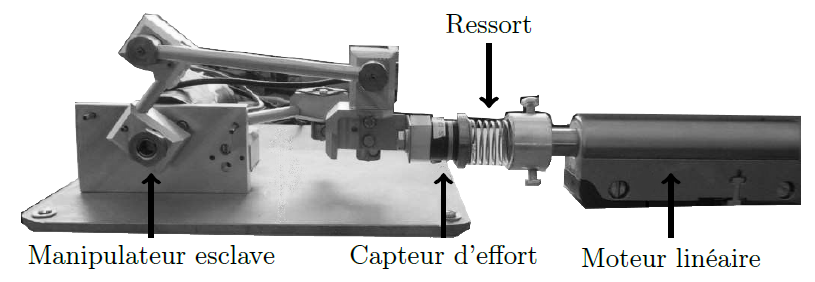
\includegraphics[width=0.7\linewidth]{img/Figure15}
\end{center}
\caption{Manipulateur esclave associé au dispositif de simulation du mouvement respiratoire}
\label{fig15}
\end{figure}

Les performances de l'asservissement dépendent (entre autres) de la qualité de la chaîne d'acquisition. Cela passe notamment par le réglage de la fréquence d'échantillonnage et la quantification du convertisseur analogique numérique.

\begin{figure}[ht!]
\begin{center}
 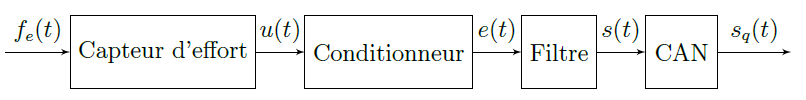
\includegraphics[width=0.7\linewidth]{img/Figure16}
\end{center}
\caption{Schéma de la chaîne d'acquisition}
\label{fig16}
\end{figure}

Il est nécessaire d'ajouter un filtre avant la Conversion Analogique Numérique.
\\ ~\ \\
\begin{minipage}{0.35\linewidth}
 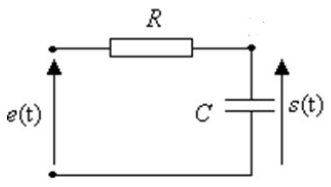
\includegraphics[width=0.9\linewidth]{img/Figure17}
\end{minipage}\hfill
\begin{minipage}{0.6\linewidth}
Ce filtre \og anti-repliement \fg est généralement réglé à la fréquence $f_0=\dfrac{f_{ech}}{2}$ où $f_{ech}$ est la fréquence d'échantillonnage qui est ici de 50 Hz.
\end{minipage}

\question{Déterminer la fonction de transfert $H_2(p)=\dfrac{S(p)}{E(p)}$ du filtre RC.}

\question{Tracer l'allure du diagramme de Bode de la fonction de transfert ainsi déterminée et calculer la pulsation de cassure $\omega_c$ en fonction de $R$ et $C$. Le tracé est à effectuer sur la copie. Les valeurs numériques n'étant pas fournies, indiquer sur le tracé le maximum d'informations disponibles. En déduire la fréquence propre $f_0$ en fonction de $R$ et $C$.}

\question{En déduire la valeur du produit $R.C$ afin de valider le réglage du filtre.}

\newpage

\subsection{Modélisation et étude des performances du système sans correction}

\paragraph{Objectif :} Identifier les performances non satisfaites afin de choisir un correcteur adapté.

La modélisation permettant de relier la consigne $x_m(t)$ issue du dispositif maître au déplacement $x_v(t)$ de l'organe terminal est représentée par le schéma bloc suivant.

\begin{figure}[ht!]
\begin{center}
 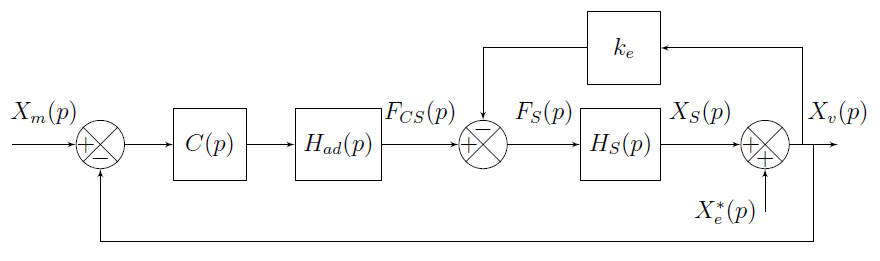
\includegraphics[width=0.9\linewidth]{img/Figure18}
\end{center}
\caption{Modélisation du dispositif esclave avec son environnement perturbé}
\label{fig18}
\end{figure}

\begin{itemize}
 \item $H_{ad}(p)=k_a=1N.m^{-1}$ permet d'adapter la consigne position en consigne force,
 \item $H_s(p)=\dfrac{X_s(p)}{F_s(p)}=\dfrac{k_s}{p.(m_s.p+b_s)}$, avec $k_s=1m.N^{-1}$, $m_s=0,152kg$ et $b_S=1,426N.s.m^{-1}$,
 \item $k_e=200N.m^{-1}$.
\end{itemize}

\question{Simplifier le schéma bloc précédant pour lui donner la forme illustrée par la figure suivante. Exprimer $H_t(p)$ et $H(p)$ en fonction de $k_e$, $k_a$ et $H_s(p)$.}

\begin{figure}[ht!]
\begin{center}
 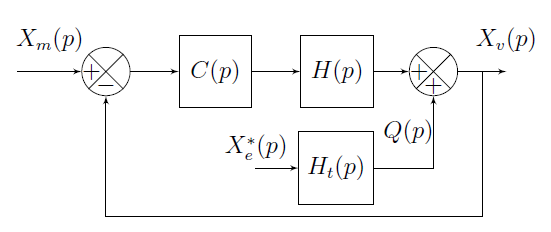
\includegraphics[width=0.6\linewidth]{img/Figure19}
\end{center}
\caption{Modélisation simplifiée du dispositif esclave}
\label{fig19}
\end{figure}

Pour la suite du problème, on prendra : $H(p)=\dfrac{1}{m_s.p^2+b_s.p+k_e}$.

\newpage

\subsection{Vérification des exigences sans correction : C(p) = 1}

\question{Déterminer la fonction de transfert en boucle fermée (avec une perturbation nulle :
$X^*_e(p)=0$): $F_{BF1}(p)=\dfrac{X_v(p)}{X_m(p)}$, puis la mettre sous forme canonique de façon à identifier les paramètres caractéristiques :}
\begin{itemize}
 \item gain statique ($K$),
 \item pulsation propre ($\omega_0$),
 \item coefficient d'amortissement ($z$). 
\end{itemize}

Faire l'application numérique.

Trois réponses ont été tracées, et l'une d'entre elles correspond à la fonction calculée précédemment.

\begin{figure}[ht!]
\begin{center}
\begin{minipage}{0.3\linewidth}
 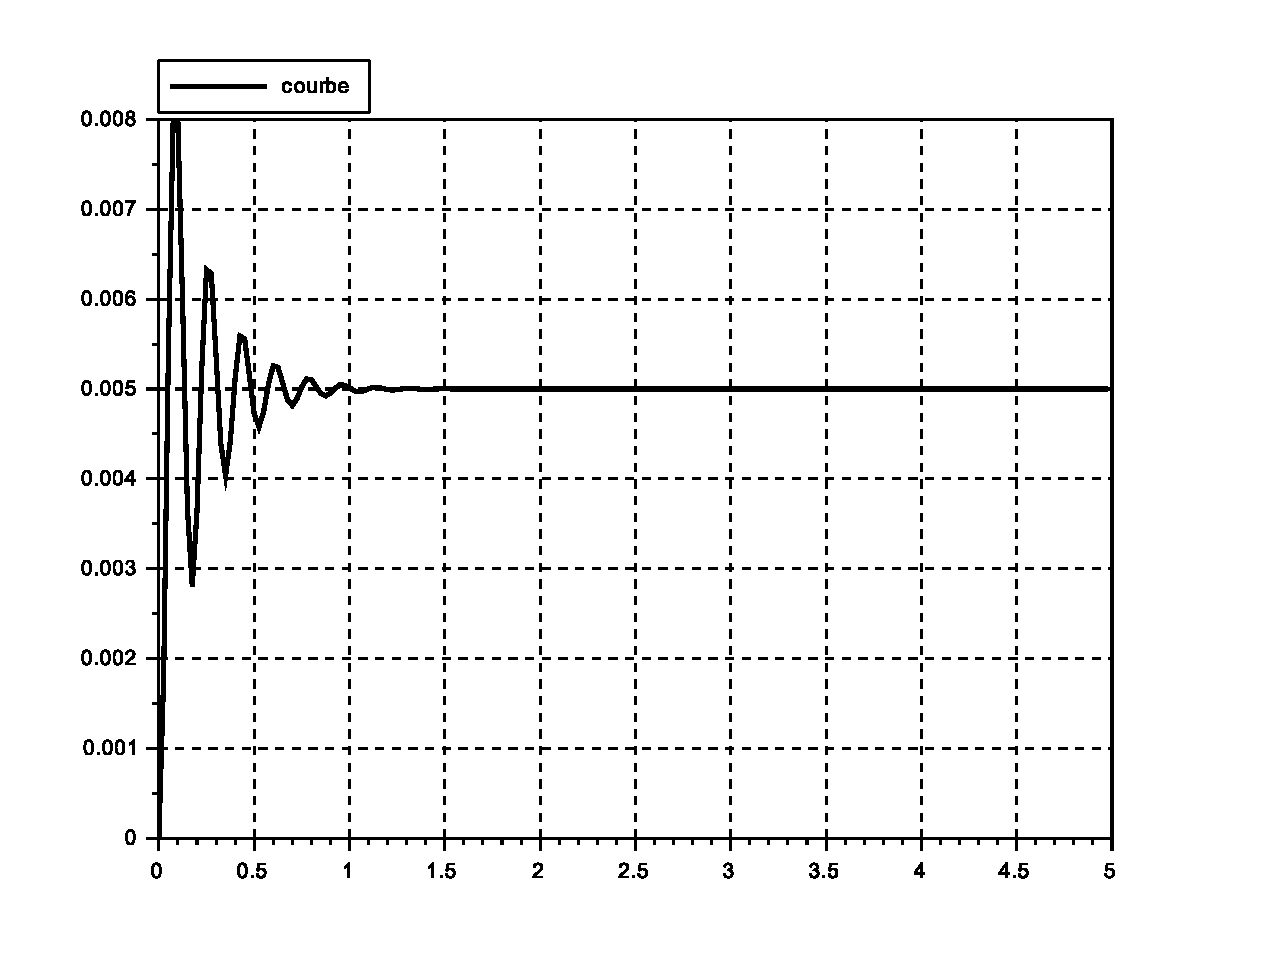
\includegraphics[width=0.8\linewidth]{img/Inf}
\end{minipage}\hfill
\begin{minipage}{0.3\linewidth}
 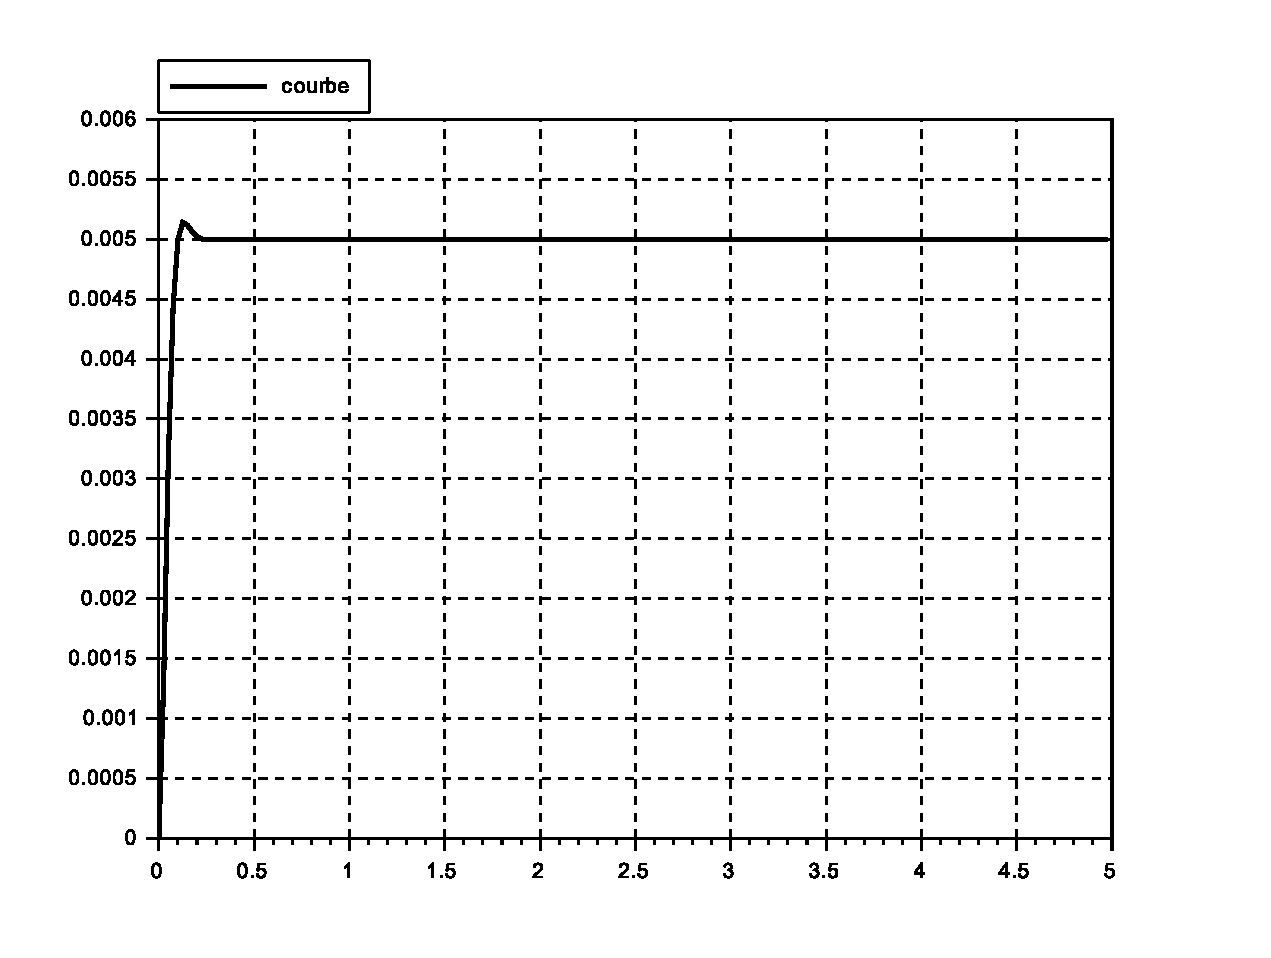
\includegraphics[width=0.8\linewidth]{img/Int}
\end{minipage}\hfill
\begin{minipage}{0.3\linewidth}
 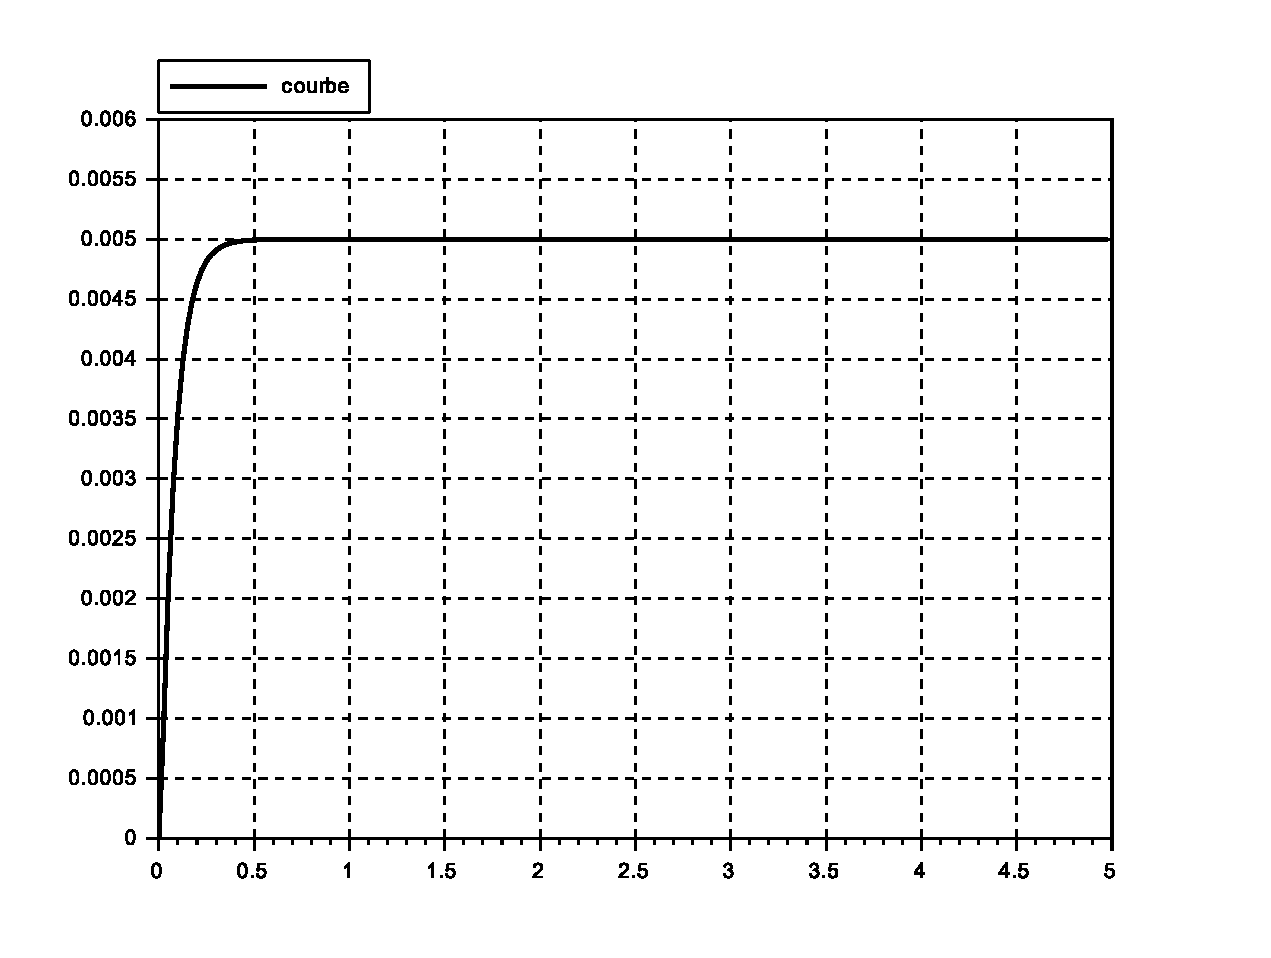
\includegraphics[width=0.8\linewidth]{img/Sup}
\end{minipage}\hfill
\end{center}
\caption{Réponses temporelles}
\label{fig20}
\end{figure}

\question{Déterminer à quel tracé correspond la fonction de transfert de la question précédente et déterminer la valeur de l'échelon qui lui a été appliqué en entrée.}

\question{En vous aidant des abaques des figures suivantes, vérifier les exigences \og stabilité \fg (uniquement l'amortissement), \og rapidité \fg et \og précision \fg (uniquement l'erreur statique).}

\begin{figure}[ht!]
\begin{center}
 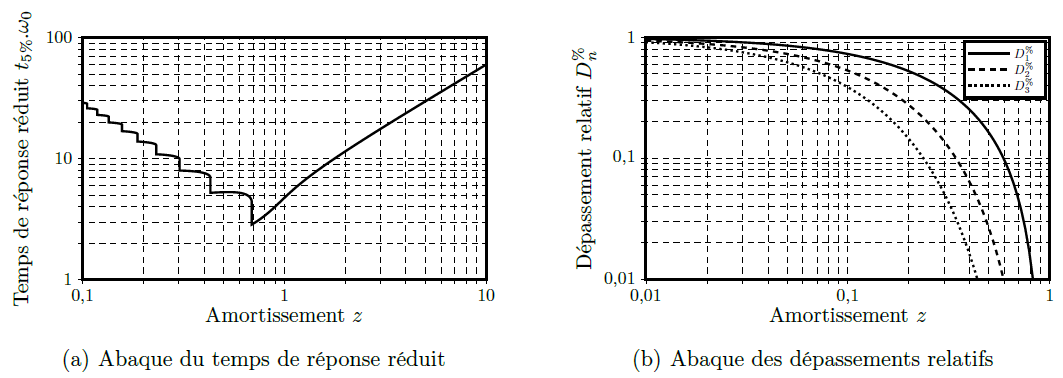
\includegraphics[width=0.8\linewidth]{img/Figure22}
\end{center}
\caption{Abaques pour un système linéaire d'ordre 2}
\label{fig22}
\end{figure}

\newpage

\section{Conception du Mécanisme de HOEKEN (50 min)}

L'assemblage du mécanisme de HOEKEN doit être démontable. Pour cela on demande de réaliser la liaison encastrement par vis du montage suivant.

\begin{minipage}{0.45\linewidth}
	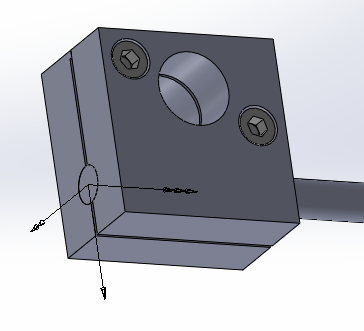
\includegraphics[width=0.7\linewidth]{img/Figure20}
\end{minipage}\hfill
\begin{minipage}{0.45\linewidth}
	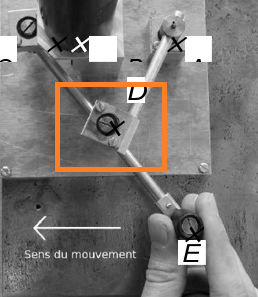
\includegraphics[width=0.7\linewidth]{img/Figure21}
\end{minipage}

\question{Proposer une solution d'assemblage par vis du système suivant. Une des deux pièces doit être taraudée, il n'est pas permis d'utiliser d'écrou. Représenter la réponse sur la vue en coupe du document réponse \og Mécanisme de HOEKEN \fg.}

\begin{center}
\huge{-- FIN --}
\end{center}

\newpage

\cleardoublepage

\newpage
\cleardoublepage

\pagestyle{documentreponse}

\section{Document réponse}

\ifdef{\public}{
\begin{tikzpicture} 
	\draw (0,0) rectangle (2,2);
	\draw (0,0) -- (2,2);
	\draw (1.5,0.5) node {\large 20};
	\draw (2.5,0) rectangle (16,2);
	\draw (4.2,1.7) node {\large Commentaires:};
\end{tikzpicture}\\} 

\reponse{9}{}{$L_2=\sqrt{(L_0+L_1.cos(\theta_1)-L_2.cos(\theta_3))^2+(L_1.sin(\theta_1)-L_2.sin(\theta_3))^2}$.}

\reponse{7}{}{$\overrightarrow{AE}=L_0.\overrightarrow{x_0}+L_1.\overrightarrow{x_1}-2.L_2.\overrightarrow{x_3}=\left(\begin{array}{c} L_0+L_1.cos(\theta_1)-2.L_2.cos(\theta_3) \\ L_1.sin(\theta_1)-2.L_2.sin(\theta_3) \\ 0
\end{array}\right)$}

\ifdef{\public}{\newpage}

\reponse{7}{}{Sur l'intervalle considéré :
\begin{itemize}
 \item Sur la figure 6.(a) on relève que $X_E$ varie de 100 mm, ce qui est supérieur à 50 mm la valeur exigée pour l'amplitude de déplacement (Id 1.2.1.1),
 \item Sur la figure 6.(b) on relève que l'amplitude en Y est $Y_E{max}-Y_E{min}=-100+100.25=0.25mm$ ce qui est inférieur à 0,5 mm la valeur maximale admissible par l'exigence de mouvement rectiligne (Id 1.2.1.2),
 \item Sur la figure 6.(b) on relève le taux de variation $-2\%<\dfrac{dY_E}{dX_E} \leq 2\% $ ce qui vérifie l'exigence de mouvement rectiligne (Id 1.2.1.2).
\end{itemize}

Ainsi le déplacement du point E est compatibles avec les exigences (Id 1.2.1.1) et (Id 1.2.1.2) sur l'intervalle $[ -60 mm, 40 mm]$.}

\reponse{11}{}{L'exigence considérée spécifie que la relation entre des déplacements doit être linéaire à 99\%.

Si la grandeur associée au déplacement du bouton de commande est clairement identifiable (c'est XE), celle associée au capteur de position est plus floue. En supposant que le capteur de position soit un capteur angulaire intercalé entre le bâti (0) et la barre (1), il s'agit alors de $\theta_1$. Ce choix est conforté par la figure donnant les évolutions de XE en fonction de $\theta_1$.

Pour vérifier l'exigence sur l'intervalle $[-60 mm, 40 mm]$, on propose d'exploiter les valeurs visibles sur le zoom donné figure 8(b) pour tracer une courbe avec un tableur. Le coefficient de corrélation de la régression linéaire devra être supérieur à $0,99$ pour vérifier l'exigence.}

\ifdef{\public}{\newpage}

\reponse{22}{}{
Isolement de 1.

Pour faire le calcul il suffit de déplacer le torseur de $3\rightarrow 1$ au point B.

Ainsi, $N_{B,31}=L_1.(cos\theta_1.Y_{31}-sin\theta_1.X_{31})$

On obtient alors pour l'isolement de 1, $L_1.(cos\theta_1.Y_{31}-sin\theta_1.X_{31})+C_m=0$

\noindent Isolement de 2.

Pour faire le calcul il suffit de déplacer le torseur de $3\rightarrow 2$ au point A.

Ainsi, $N_{A,32}=L_2.(cos\theta_2.Y_{32}-sin\theta_2.X_{32})=0$

On obtient alors pour l'isolement de 2, $cos\theta_2.Y_{32}-sin\theta_2.X_{32}=0$

\noindent Isolement de 3

Pour faire le calcul il suffit de déplacer les torseurs de $1\rightarrow 3$ et de $Op\rightarrow 3$ au point D.

\noindent Moment statique

Ainsi, $N_{B,Op3}=-L_2.(cos\theta_3.Y_{31}-sin\theta_3.X_{31})$ et $N_{B,Op3}=L_2.F.sin\theta_3$.

On obtient alors pour l'isolement de 3 et par application du théorème du moment $-L_2.(cos\theta_3.Y_{31}-sin\theta_3.X_{31})+L_2.F.sin\theta_3=0$, donc $sin\theta_3.X_{31}+F.sin\theta_3-cos\theta_3.Y_{31}=0$

\noindent Résultante statique

Ainsi, $Y_{13}=sin\theta_2.X_{31}-cos\theta_2.Y_{31}$.

On obtient alors pour l'isolement de 3 et par application du théorème de la résultante $-F.sin\theta_2+sin\theta_2.X_{31}-cos\theta_2.Y_{31}=0$
}

\reponse{8}{}{L'exigence \og Linéarité couple/effort \fg (id 1.3.2.2) impose d’avoir le ratio couple/effort constant à $\pm1\%$.

Le zoom de la figure 9(b) donne $\left(\frac{C}{F}\right)_{max}=33.375 mm$ et $\left(\frac{C}{F}\right)_{min}=32.75 mm$

$\frac{\left(\frac{C}{F}\right)_{max}-\left(\frac{C}{F}\right)_{min}}{\left(\frac{C}{F}\right)_{min}}=\frac{33.375-32.75}{32.75}=\frac{33.75-32.75}{32.75}=\frac{0.625}{32.75}<2\%$, donc la condition est respectée.}

\reponse{8}{}{Ce codeur délivre 4000 impulsions par tour (2 impulsions par fente et par capteur). 

Il a donc une résolution de $\frac{360}{4000}=0.09$\textdegree$.pt^{-1}$ de mesure.

La figure 8(b) nous donne le coefficient de proportionnalité :

$\frac{\Delta X_E}{\Delta\theta 1}=\frac{38-(-55)}{260-100}=\frac{93}{160}=0,581mm.$\textdegree$^{-1}$

Pour une rotation de $0.09$\textdegree du moteur correspond un déplacement du point E de :

$\Delta X_E=0,581*0.09=0,052mm$

Cette valeur est inférieure à $0.1mm$ imposée par l’exigence (id : 1.2.2.1) qui est donc satisfaite.
}

\ifdef{\public}{\newpage}

\reponse{3}{
\begin{center}
 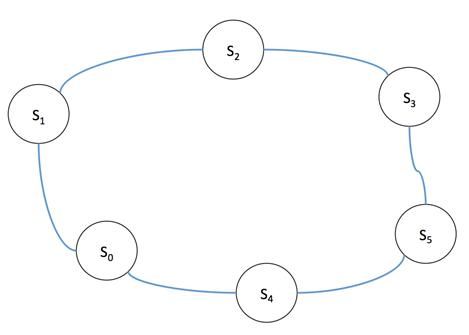
\includegraphics[width=0.8\linewidth]{img/liaisons_vierge}
\end{center}
}{
~\ \\
\begin{minipage}{0.45\linewidth}
	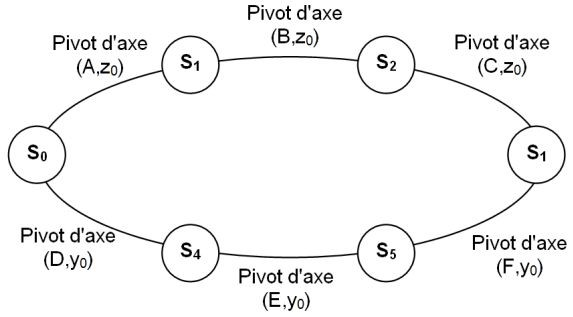
\includegraphics[width=0.9\linewidth]{img/liaisons}
\end{minipage}\hfill
\begin{minipage}{0.45\linewidth}
\begin{itemize}
 \item Formule de mobilité : $h = N_s-r_s$,
 \item $N_s = 6\times 5=30$ (6 pivots),
 \item $r_s = 6\times (6-1)-1 = 29$,
 \item $h = 1$
\end{itemize}
\end{minipage}}

\reponse{7}{}{

Pour obtenir $h=0$ à partir de $h=1$, il faut ajouter un degré de liberté sans augmenter la mobilité.

La solution la plus naturelle est de remplacer un pivot par un pivot glissant. Seulement ce n'est pas la bonne car cela rajoute une mobilité.

Ceci fait on s'aperçoit qu'il faut alors modifier une liaison en ajoutant une rotation ne modifiant pas la mobilité globale. Par exemple on peut ajouter à $L_{12}$ pivot d'axe $(B,\overrightarrow{z_0})$ la rotation d'axe $(B,\overrightarrow{x_0})$, ce qui la transforme en une sphérique à doigt.}

\reponse{10}{}{

En considérant la chaîne de solides (0-1-2-3), on a :

$\overrightarrow{\Omega(3/0)}=\omega_{30}.\overrightarrow{z_0}$, et par suite, $\overrightarrow{V(C,3/0)}\in$ plan $(A,\overrightarrow{x_0},\overrightarrow{y_0})$.

En considérant la chaîne de solides (0-4-5-3), on a :

$\overrightarrow{\Omega(3/0)}=\omega_{30}.\overrightarrow{y_0}$, et par suite, $\overrightarrow{V(C,3/0)}\in$ plan $(A,\overrightarrow{x_0},\overrightarrow{z_0})$.

Pour le mécanisme dans son ensemble, les mobilités doivent être compatibles :

$\overrightarrow{\Omega(3/0)}=\omega_{30}.\overrightarrow{z_0}=\omega_{30}.\overrightarrow{y_0}$, donc $\overrightarrow{\Omega(3/0)}=\overrightarrow{0}$

$\overrightarrow{V(C,3/0)}\in$ plan $(A,\overrightarrow{x_0},\overrightarrow{y_0})$ et $\overrightarrow{V(C,3/0)}\in$ plan $(A,\overrightarrow{x_0},\overrightarrow{z_0})$, donc $\overrightarrow{V(C,3/0)}$ // $\overrightarrow{x_0}$.

Finalement $\left\{V(3/0)\right\}=\left\{\begin{array}{c}\overrightarrow{\Omega(3/0)}=\overrightarrow{0} \\ \overrightarrow{V(C,3/0)}=V(C,3/0).\overrightarrow{x_0}\end{array}
\right\}$ donc M(3/0) est une translation selon $\overrightarrow{x_0}$.}

\reponse{10}{}{
$\overrightarrow{V(C,3/0)}=\overrightarrow{V(C,3/2)}+\overrightarrow{V(C,2/1)}+\overrightarrow{V(C,1/0)}=\overrightarrow{CB}\wedge \overrightarrow{\Omega(2/1)}+\overrightarrow{CA}\wedge \overrightarrow{\Omega(1/0)}$

$\overrightarrow{V(C,3/0)}=-L_2.(cos(\theta_2).\overrightarrow{x_0}+sin(\theta_2).\overrightarrow{y_0})\wedge \dot{\theta_2}.\overrightarrow{z_0}-(L_2.(cos(\theta_2).\overrightarrow{x_0}+sin(\theta_2).\overrightarrow{y_0})+L_1.(cos(\theta_1).\overrightarrow{x_0}+sin(\theta_1).\overrightarrow{y_0}))\wedge \dot{\theta_1}.\overrightarrow{z_1}$

$\left\{\begin{array}{l} L_2.\dot{\theta_2}.sin(\theta_2)+L_2.\dot{\theta_1}.sin(\theta_2)+L_1.\dot{\theta_1}.sin(\theta_1)=0 \\ V_c=L_2.\dot{\theta_2}.cos(\theta_2)+L_2.\dot{\theta_1}.cos(\theta_2)+L_1.\dot{\theta_1}.cos(\theta_1)
\end{array}\right.$

Donc,
$V_c=-\left(cos\theta_1+\frac{sin\theta_1}{tan\theta_2}\right).L_1.\dot{\theta_1}$}

\reponse{10}{}{Transformée de Laplace

$\left[\left(M_3+I_1.\alpha^2\right).p^2+f.\alpha^2.p\right]X_s(p)=C_m(p).\alpha$, d'où

$H(p)=\dfrac{\dfrac{1}{f.\alpha}}{p.\left(\dfrac{(M_3+I_1\alpha^2)}{f.\alpha^2}.p+1 \right)}$

A.N: $H(p)=\dfrac{-20,8}{p.(0,1.p+1)}$}

\reponse{9}{}{
~\ \\

Il faut considérer la figure, et la fin de la phase d'insertion. Compte-tenu de ce qui est demandé (relation linéaire), on va retenir la phase entre les instants $t_1$ et $t_2$ sur l'extrait de la figure ci-contre. \\
Durant cette phase, les grandeurs $f_e$ et $x_e$ ont toutes deux une évolution linéaire. De plus $x_e=0$ quand $f_e=0$.

$k_e=\dfrac{0,5}{0,03}=16,6N.m^{-1}$
}

\reponse{9}{}{

L'évolution de $x_e(t)$ est périodique et apparemment sans discontinuité de tangente. On peut donc la modéliser par une sinusoïde. On relève sa période $T=4,25s$ environ.

Son amplitude est  $\Delta x_e=0mm-(-10)mm=+10mm$.

Sa valeur moyenne est non nulle et on relève $x_{e0}=-5mm$.

Enfin $x_e(0)\neq x_{e0}$ donc la fonction sinus possède une phase non nulle à l'origine.

D'où l'expression de la fonction $x_e(t)=x_{e0}+\dfrac{\Delta x_e}{2}.sin(\omega.t+\phi)$

En remplaçant par les valeurs numériques de déplacement, et $\omega=2.\pi.f=\dfrac{2.\pi}{T}$ il vient : $x_e(t)=-5.10^{-3}+5.10^{-3}.sin(2.\pi.f.t+\phi)=5.10^{-3}.[-1+sin(2.\pi.f.t+\phi)]$. CQFD.

On identifie $A=5mm$ et $f=\dfrac{1}{T}=0.24Hz$.

Finalement, $f_e(t)=k_e\times x_e(t)=\left[-1+sin\left(2.\pi.\dfrac{t}{4,25}+\phi\right)\right]$}

\reponse{6}{}{

La fonction de transfert est $H_2(p)=\dfrac{1}{1+R.C.p}$
}


\ifdef{\public}{\newpage}

\reponse{3}{
\begin{center}
 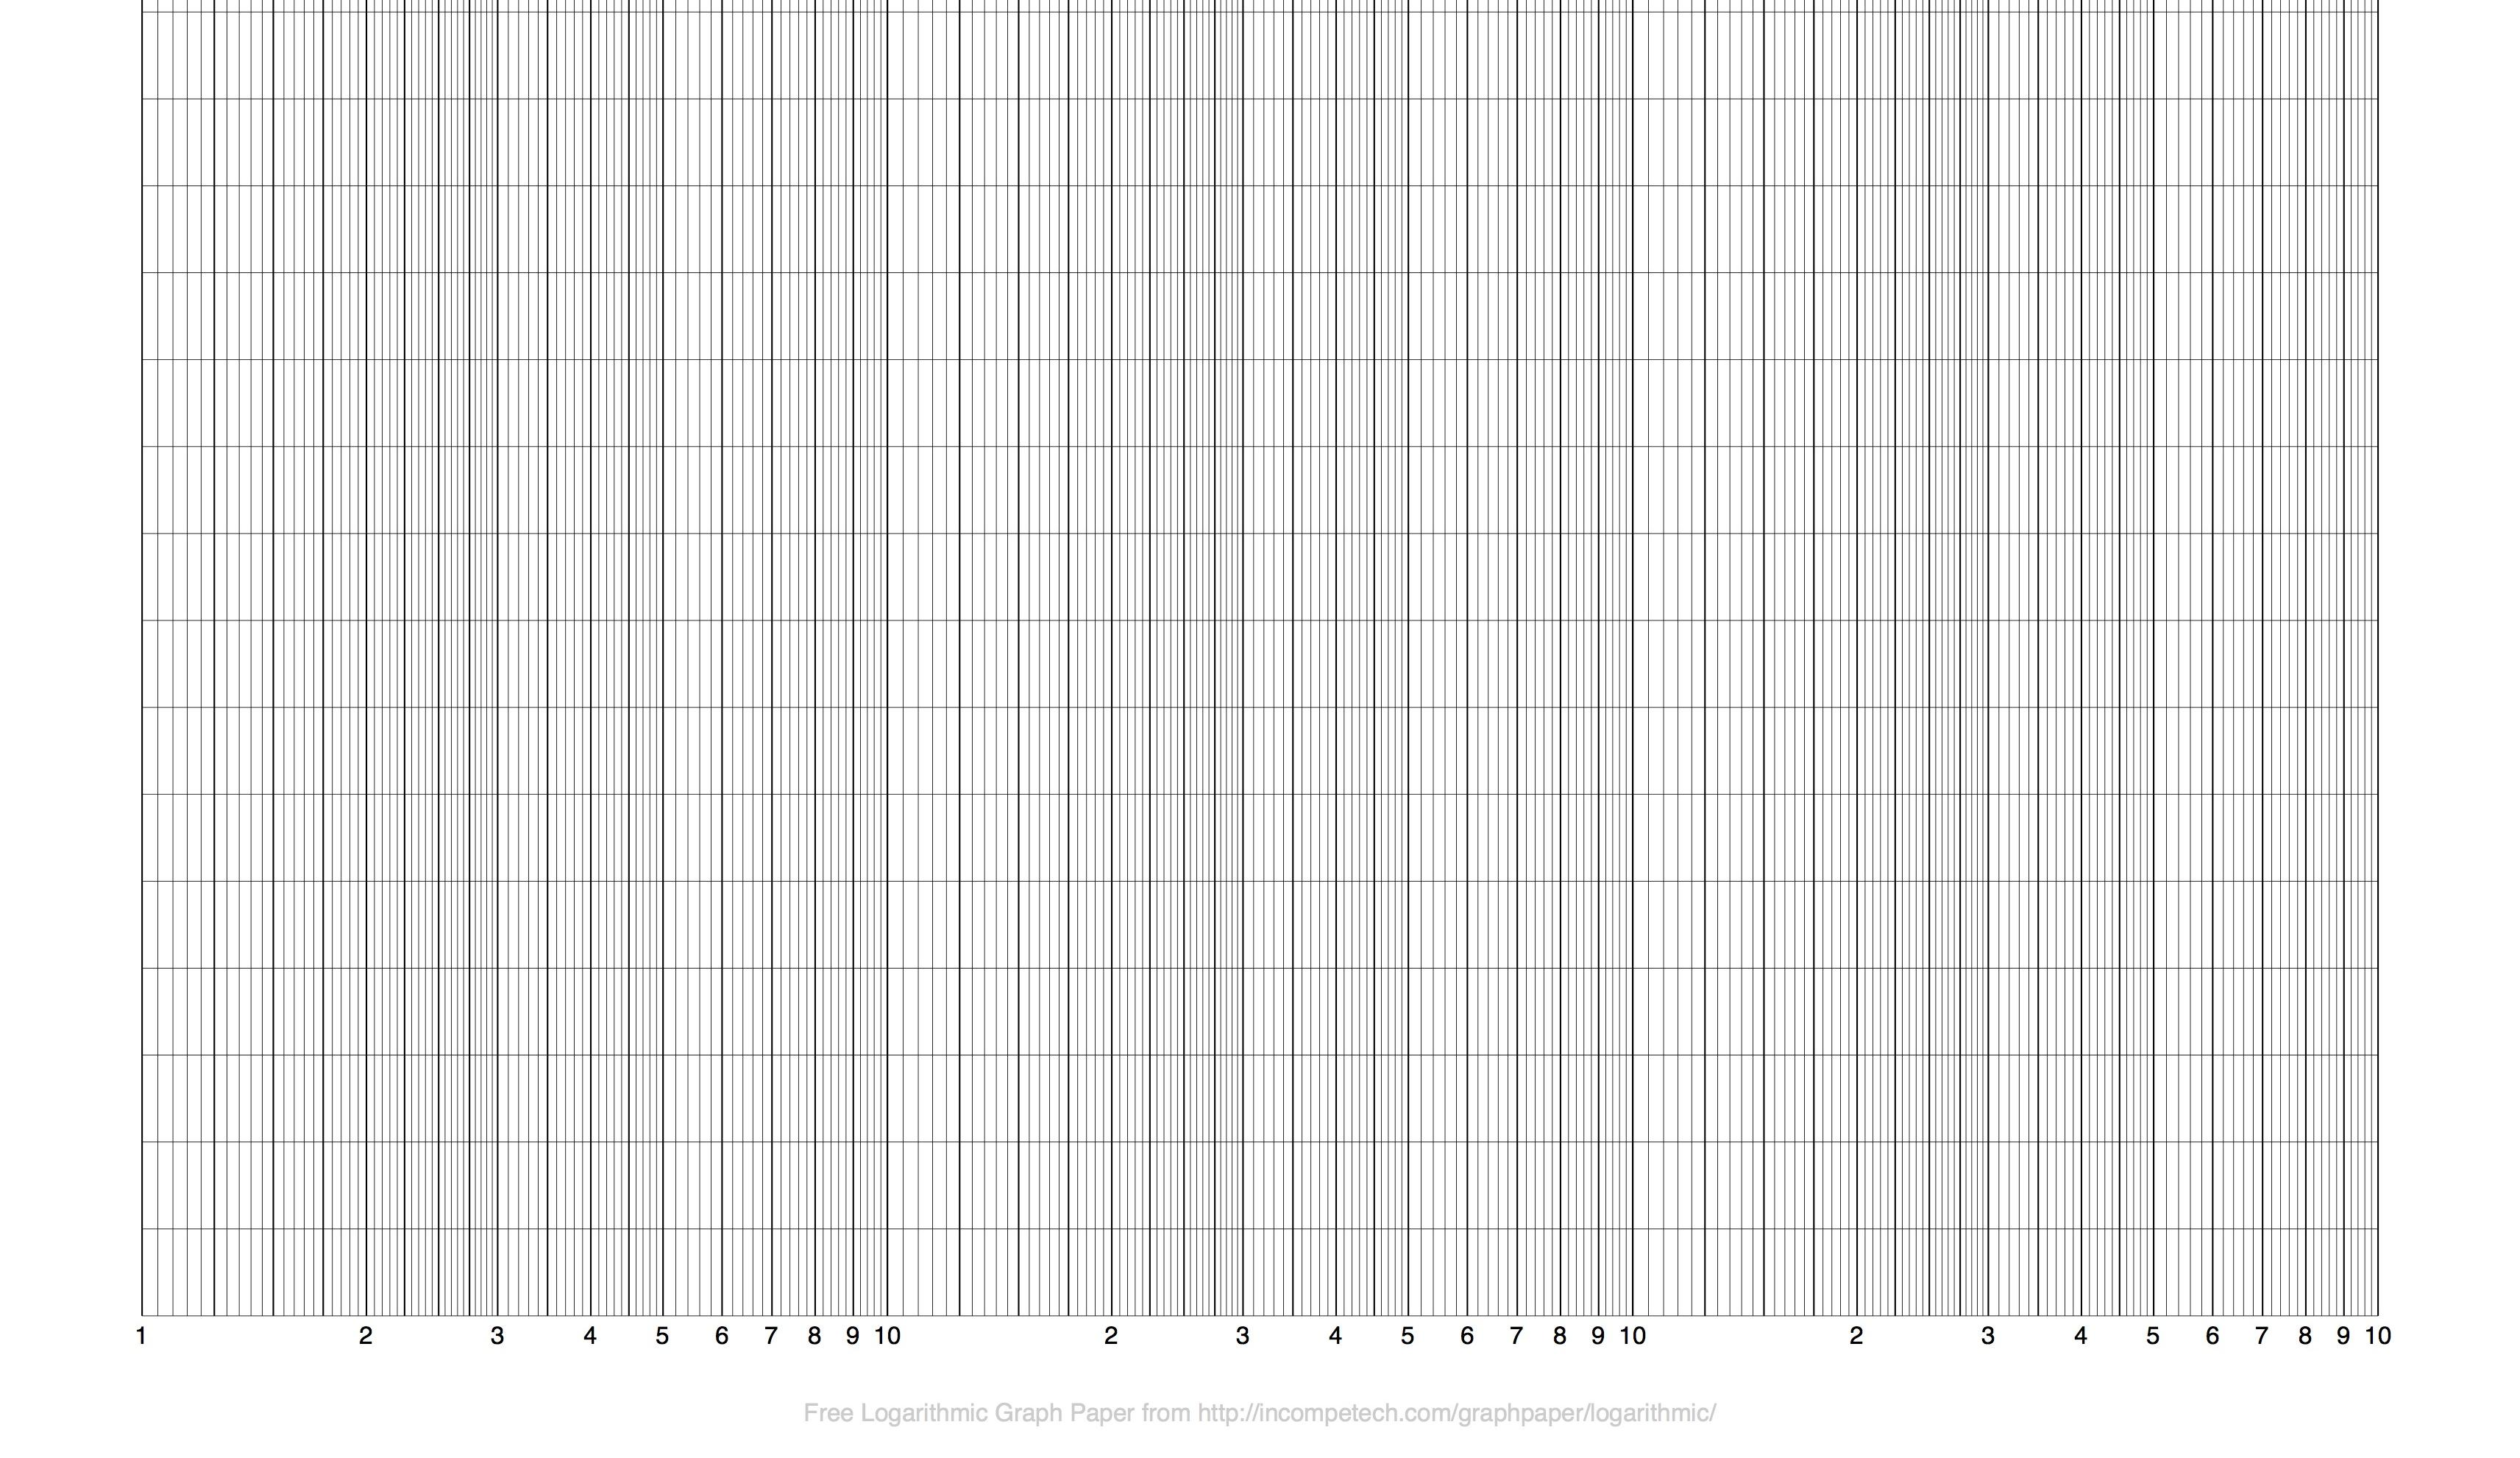
\includegraphics[width=0.8\linewidth]{img/Bode_vierge}\\
 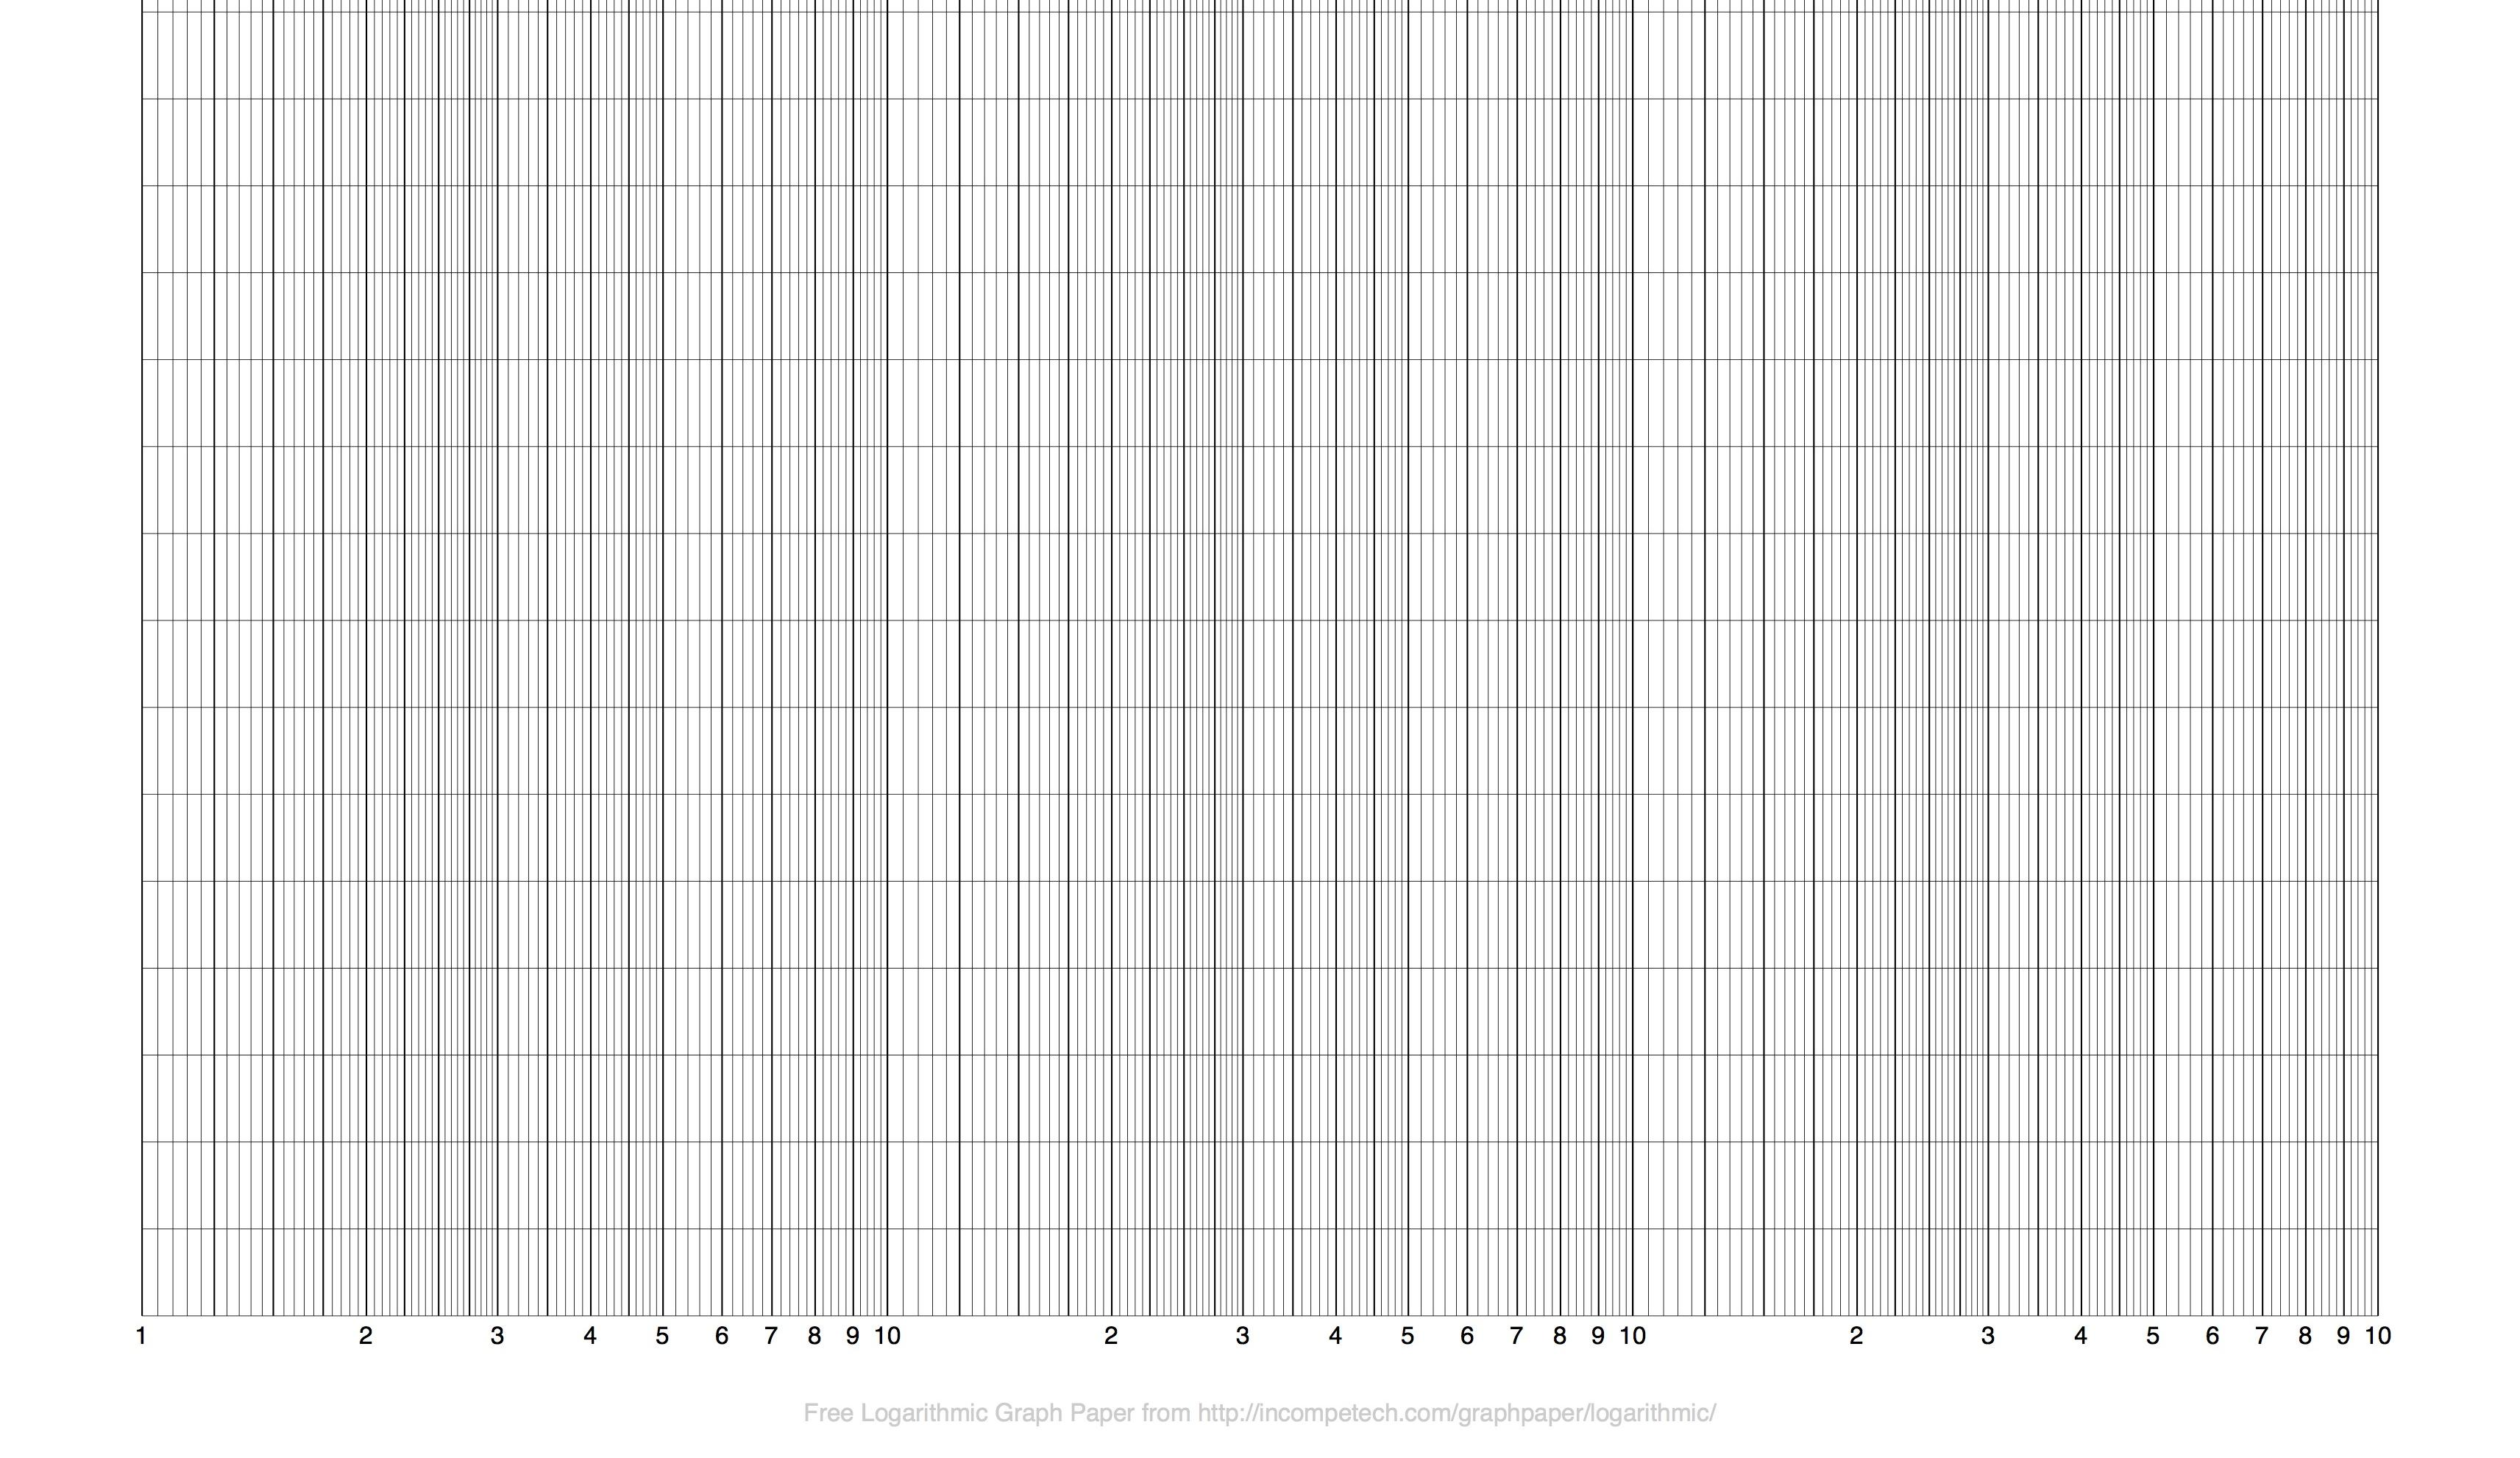
\includegraphics[width=0.8\linewidth]{img/Bode_vierge}
\end{center}
}{
 ~\ \\

\begin{center}
 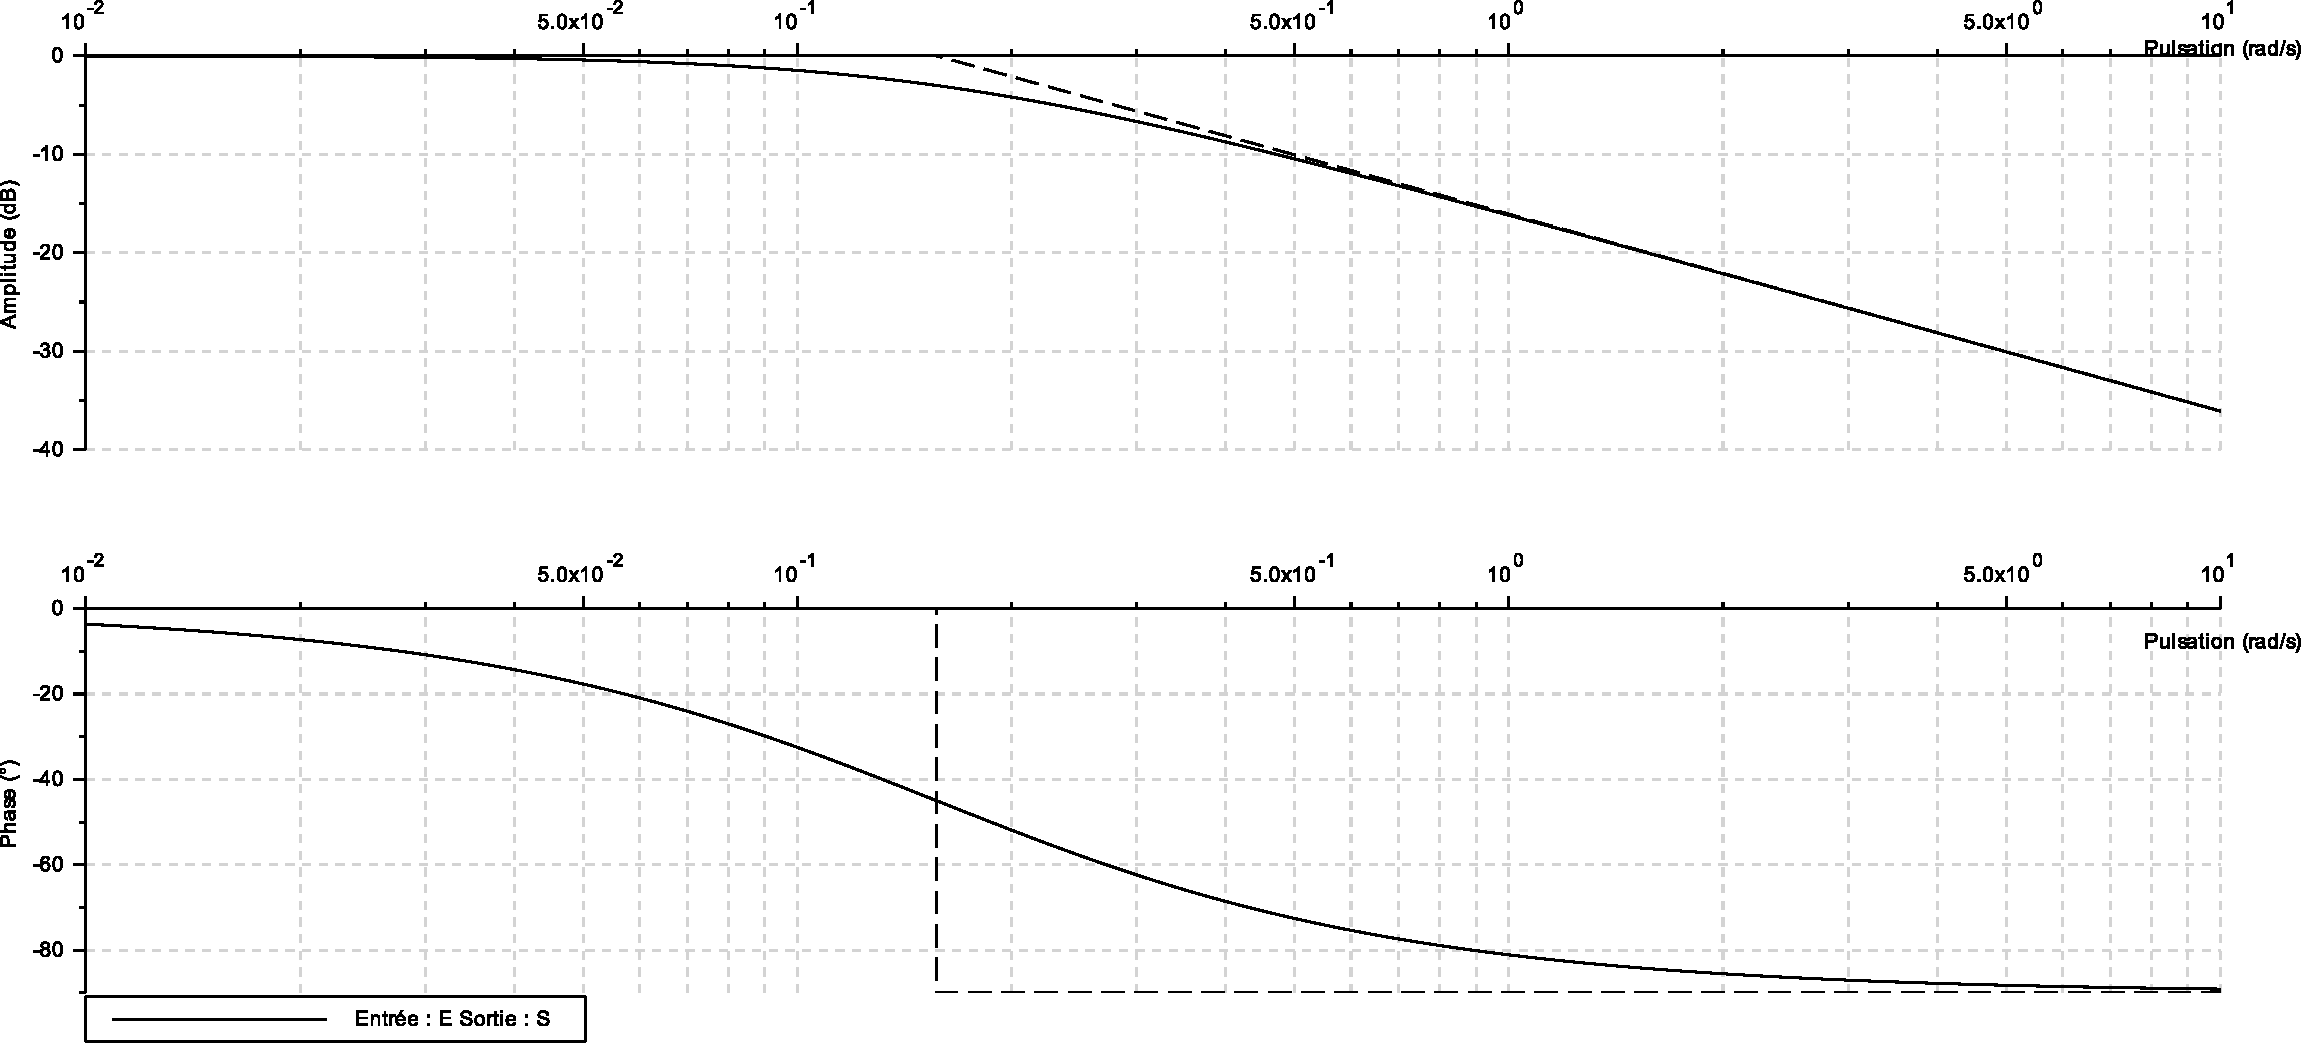
\includegraphics[width=0.7\linewidth]{img/Bode}
\end{center}

Sa pulsation propre est égale à sa pulsation de cassure $\omega_0=\omega_c=\dfrac{1}{\tau}=\dfrac{1}{R.C}$, d'où la fréquence propre $f_0=\dfrac{\omega_0}{2.\pi}=\dfrac{1}{2.\pi.R.C}$.}

\ifdef{\public}{\newpage}

\reponse{2}{}{

On impose $f_0=\dfrac{f_{ech}}{2}$ d'où finalement $\dfrac{f_{ech}}{2}=\dfrac{1}{2.\pi.R.C}$, donc $RC=\dfrac{1}{\pi.f_{ech}}$, A.N: $RC=\dfrac{1}{50.\pi}=6,37ms$
}

\reponse{3}{}{

\begin{center}
 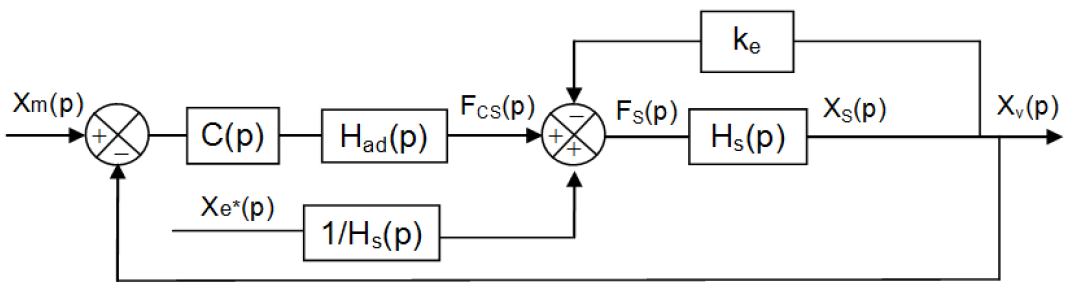
\includegraphics[width=0.7\linewidth]{img/sb1} \\
 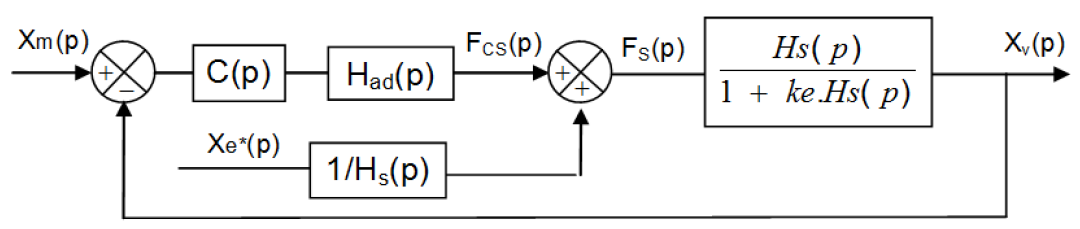
\includegraphics[width=0.7\linewidth]{img/sb2} \\
 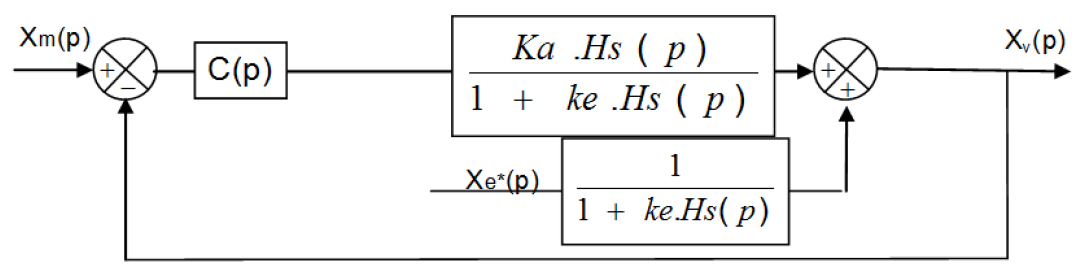
\includegraphics[width=0.7\linewidth]{img/sb3}
\end{center}

On identifie finalement : $H(p)=\dfrac{K_a.H_s(p)}{1+k_e.H_s(p)}$ et $Ht(p)=\dfrac{1}{1+k_e.H_s(p)}$.
}

\reponse{7}{}{

$F_{BF1}(p)=\dfrac{\dfrac{1}{1+k_e}}{\dfrac{m_s}{1+k_e}.p^2+\dfrac{b_s}{1+k_e}.p+1}$

\begin{itemize}
 \item Gain statique: $K=\dfrac{1}{1+k_e}=0,005$,
 \item Pulsation propre: $\omega_0=\sqrt{\dfrac{1+k_e}{m_s}}=36,4rad.s^{-1}$,
 \item Coefficient d'amortissement: $z=\dfrac{b_s}{2.\sqrt{m_s.(1+k_e)}}=0,13$.
\end{itemize}}

\reponse{3}{}{

Le tracé de la question 16 est le premier et l'échelon était unitaire.}

\ifdef{\public}{\newpage}

\reponse{5}{}{

\begin{itemize}
 \item La FT a un coefficient d'amortissement $z=0,13<1$, donc la réponse indicielle présentera un dépassement transitoire. L'exigence de stabilité (amortissement) n'est donc pas vérifiée,
 \item L'exigence rapidité impose un temps de réponse à 5\% max pour un échelon de 0,1s. Pour $z=0,13$ l'abaque du temps de réponse réduit donne $tr_{5\%}.\omega_0>20$. Ainsi $tr_{5\%}>\dfrac{20}{\omega_0}$, or $\omega_0=36,4rad.s^{-1}$ d'où $tr_{5\%}>0,55s$. L'exigence de rapidité n'est donc pas vérifiée.
 \item L'exigence de précision impose une erreur statique max relative à un échelon de 1\%. La FT ayant un gain statique K on aura en régime permanent (statique) : $\Delta_s=K.\Delta_e$, d'où une erreur statique relative : $\dfrac{\Delta_e-\Delta_s}{\Delta_e}=1-\dfrac{\Delta_s}{\Delta_e}=1-K$.	
Avec $K=0,005$ on obtient une erreur de $0,995$ bien supérieur à $1\%=0,01$. L'exigence de précision n'est donc pas vérifiée.
\end{itemize}}

\newpage

\reponse{}{\vspace{-0.5cm}\begin{center}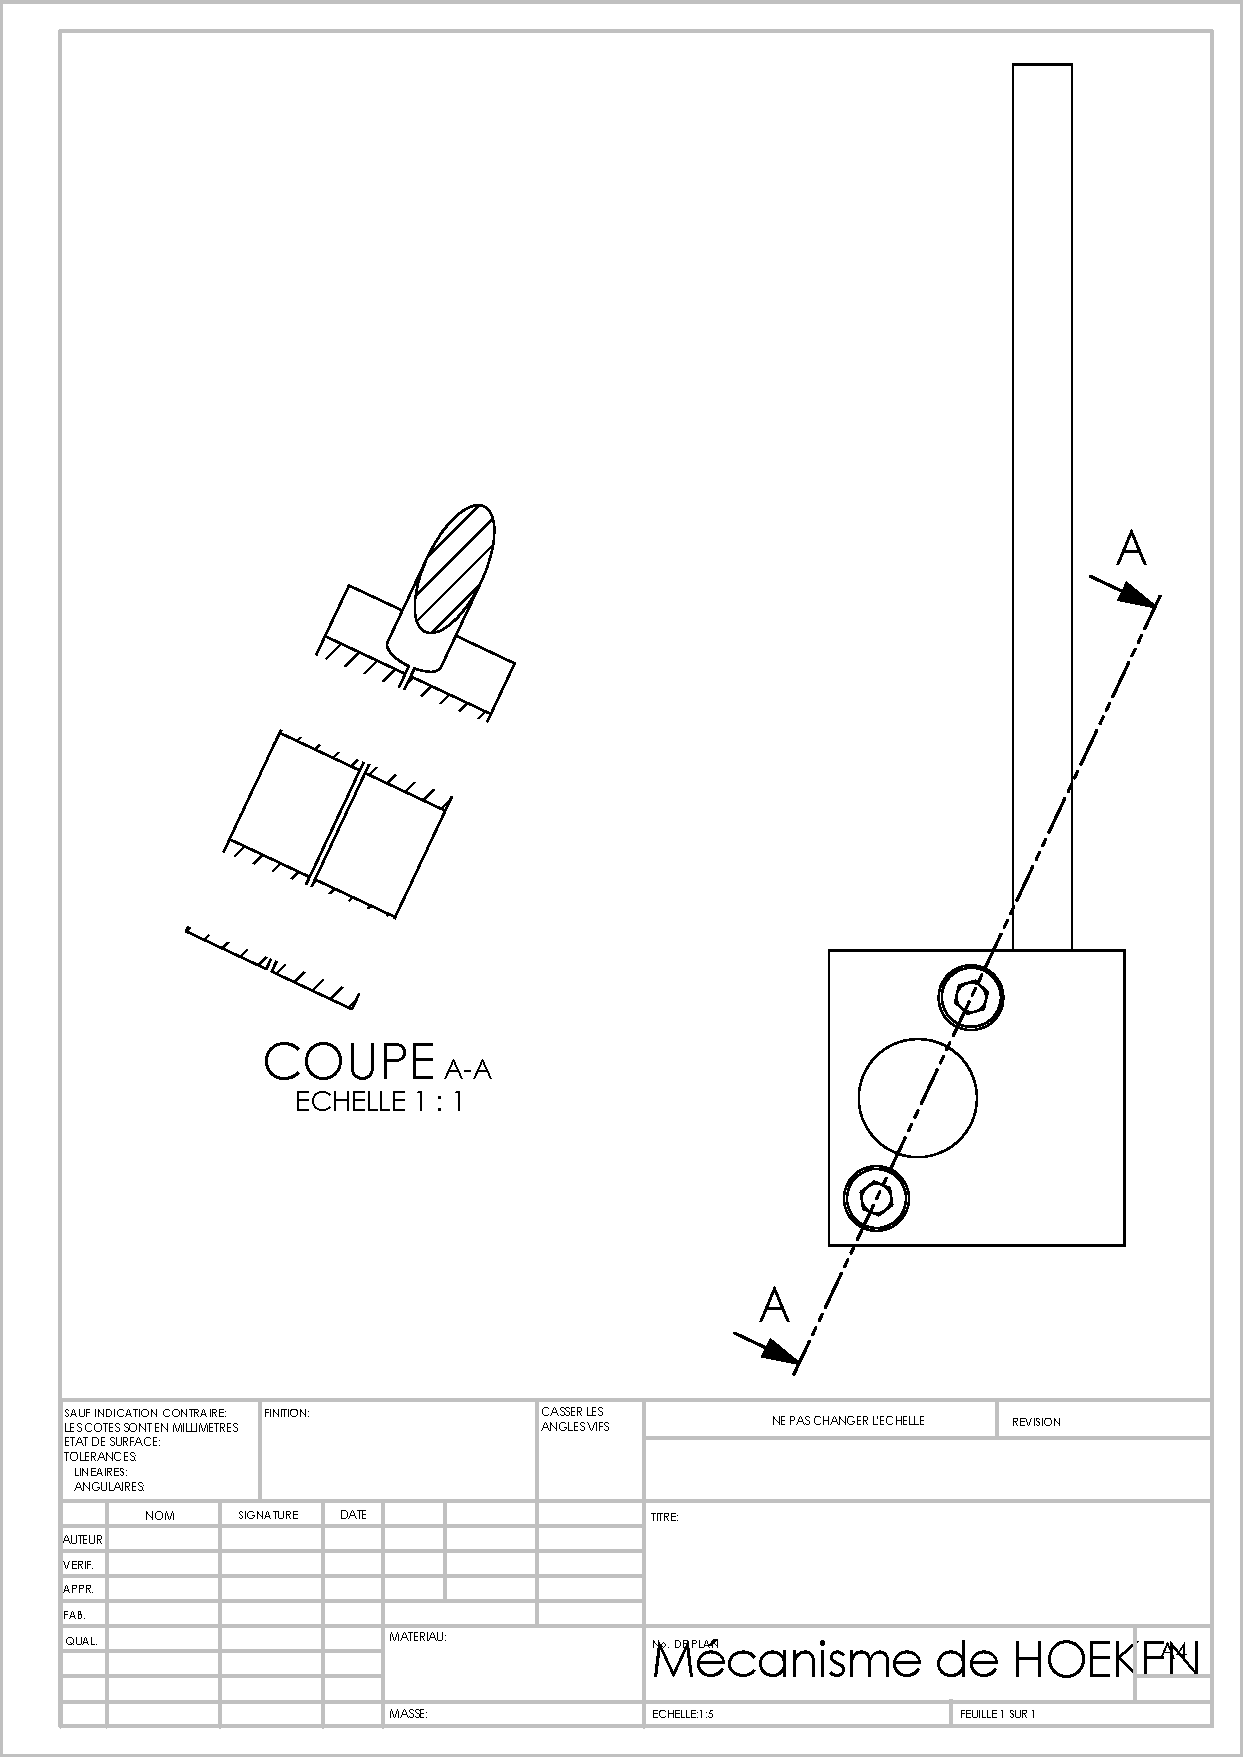
\includegraphics[width=0.9\linewidth]{img/Mecanisme_completer}\end{center}\vspace{-0.5cm}}{
\vspace{-0.5cm}\begin{center}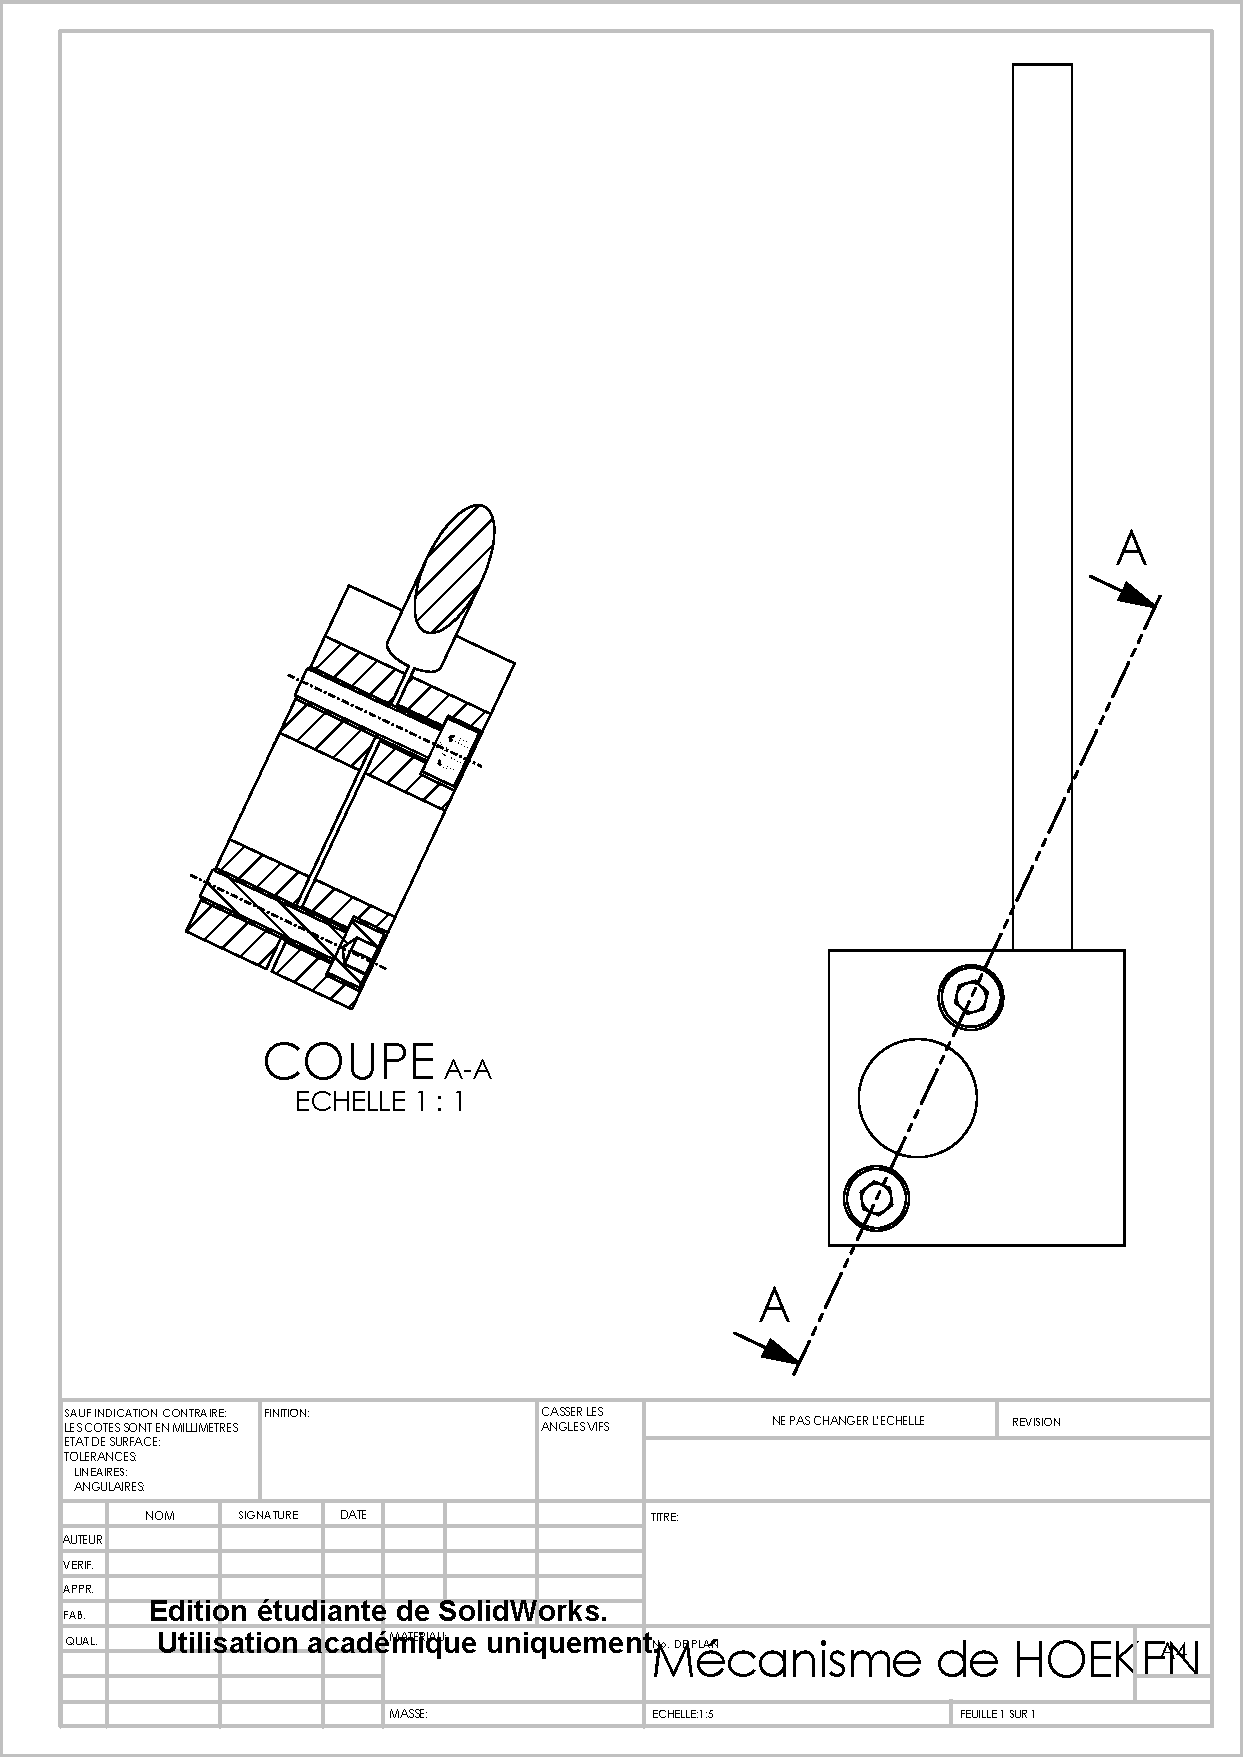
\includegraphics[width=0.9\linewidth]{img/Mecanisme_corrige}\end{center}\vspace{-0.5cm}}

\end{document}

